\documentclass[lettersize,journal]{IEEEtran}
\usepackage{amsmath,amsfonts}%√
%\usepackage{algorithmic}
\usepackage{array}%√
\usepackage[caption=false,font=normalsize,labelfont=sf,textfont=sf]{subfig}%√
\usepackage{textcomp}%√
\usepackage{stfloats}%√
\usepackage{amssymb}
\usepackage{url}%√
\usepackage{CJKutf8}
\usepackage{multirow}
\usepackage{booktabs}
\usepackage{verbatim}%√
\usepackage{graphicx}%√
\usepackage{epstopdf}
\usepackage{algorithm, algorithmicx, algpseudocode}
\hyphenation{op-tical net-works semi-conduc-tor IEEE-Xplore}
\def\BibTeX{{\rm B\kern-.05em{\sc i\kern-.025em b}\kern-.08em
    T\kern-.1667em\lower.7ex\hbox{E}\kern-.125emX}}
\usepackage{balance}
\usepackage{hyperref}
\hypersetup{hypertex=true,
	colorlinks=true,
	linkcolor=blue,
	anchorcolor=blue,
	citecolor=blue}
\usepackage{pifont} 
% \usepackage[perpage]{footmisc}  每页重新编号用的，但在表或算法框里不起作用

\begin{document}
\begin{CJK}{UTF8}{gbsn}
\title{GNN-Assisted Deep Reinforcement Learning for Cell-Free Massive MIMO Systems with Nonlinear Power Amplifiers and Low-Resolution ADCs}
\author{Meng Zhou, \textit{Member}, \textit{IEEE}, Shilong Li, Peiyan Yuan, \textit{Senior Member}, \textit{IEEE}, Junna Zhang, \textit{Member}, \textit{IEEE}, Longxiang Yang, and Hongbo Zhu
\thanks{M. Zhou, S. Li, P. Yuan, and J. Zhang are with the School of Computer and Information Engineering, Henan Normal University, Xinxiang, Henan 453007, China, and also with the Engineering Laboratory of Intellectual Business and Internet of Things Technologies, Xinxiang, Henan 453007, China (e-mail: zhoumeng@htu.edu.cn; lz13526112262@163.com; peiyan@htu.cn; zhangjunna@htu.edu.cn).

L. Yang and H. Zhu are with the Department of Communication and Information Engineering, Nanjing University of Posts and Telecommunications, Nanjing 210003, China (e-mail: yanglx@njupt.edu.cn; zhb@njupt.edu.cn).
}}
\markboth{Journal of \LaTeX\ Class Files,~Vol.~18, No.~9, September~2024}%
{How to Use the IEEEtran \LaTeX \ Templates}

\maketitle

\begin{abstract}
In cell-free massive multiple-input multiple-output (CF-mMIMO) systems, seamless communication coverage is achieved through the dense deployment of numerous access points (APs), significantly enhancing spectral efficiency (SE) for users and overall system capacity. However, the implementation of this approach demands substantial deployment costs and unavoidably necessitates the use of non-ideal hardware. This paper investigates the achievable rate of users in the uplink CF-mMIMO systems that employ nonlinear power amplifiers (PAs) and low-resolution analog-to-digital converters (ADCs) at user equipment (UE) and APs, respectively. In particular, we derive a closed-form expression for the achievable uplink user rate and conduct a comprehensive analysis of various factors, including the number of APs, UE density, number of AP antennas, and ADC resolution. To mitigate the interference among UEs and maximize the sum rate, we propose a graph neural network (GNN) assisted actor-critic algorithm (DMAGNN-AC) for power allocation. The established framework overcomes the representation bottleneck of DRL in high-dimensional unstructured state spaces and provides physically interpretable feature embeddings. In comparison to the full power output, the proposed power allocation scheme is capable of doubling the rate. Furthermore, to address the detrimental impact of low-resolution ADCs on the rate, we develop an enhanced algorithm, multi-agent deep Q-integrated network (MADQIN), which optimizes the allocation strategy of ADC resolutions. Finally, the effectiveness of the proposed schemes is validated by the presented simulation results.
\end{abstract}

\begin{IEEEkeywords}
Cell-free massive MIMO, deep reinforcement learning, graph neural network, low-resolution ADC, nonlinear power amplifier, power allocation.
\end{IEEEkeywords}


\section{Introduction}
\IEEEPARstart{C}{ELL}-FREE massive multiple-input multiple-output (CF-mMIMO) system, as an important innovation beyond fifth-generation (5G) and sixth-generation (6G), has attracted widespread attention from both academia and industry \cite{paperI1}, \cite{paperI2}. This system demonstrates great potential in the modern communication field due to its significant spectral efficiency (SE) advantage compared with traditional massive MIMO \cite{paperI3}. The core idea of the CF-mMIMO system is to provide services for a small number of user equipments (UEs) through a large number of access points (APs) distributed in various geographical locations using the same time-frequency resources \cite{paperI4}, \cite{paperI5}. This distributed architecture enables the system to make full use of diversity gains, reduces the cross-cell interference that inevitably exists in traditional massive MIMO \cite{paperI6}, and provides consistently good service quality for UEs. For these superiority, CF-mMIMO is considered one of the most promising communication technologies \cite{paperI7}.

Triggered by these significant advantages mentioned earlier, numerous studies have explored CF-mMIMO systems from various perspectives. Specifically, the achievable user rates for both the uplink and downlink were derived based on maximum ratio combining (MRC) and conjugate beamforming (CB) in \cite{paperI3}. In addition, a max-min power control algorithm was employed to provide uniform and high-quality service throughout the service area. In \cite{paperI8}, a low-complexity beamforming power allocation algorithm was proposed, utilizing CB and zero-forcing (ZF) linear precoding schemes, to boost user throughput. Furthermore, the authors of \cite{paperI7} and \cite{paperI9} individually conducted energy efficiency (EE) studies on the downlink based on CB and ZF precoding, respectively. 

However, it is noteworthy that, in addition to the aforementioned studies, more research has been conducted under ideal hardware conditions. In CF-mMIMO systems, due to the massive deployment of APs, hardware costs and power consumption grow linearly as a function of the number of antennas \cite{paperIA15}. On the one hand, a feasible solution is to replace high-precision instruments with low-cost transceivers \cite{paperI10}. Nevertheless, in practical applications, this means that the radio frequency (RF) chain hardware is susceptible to various damages. On the other hand, using low-resolution analog-to-digital converters (ADCs) is an effective way to achieve low-cost and energy-saving CF-mMIMO systems \cite{paperI11}-\cite{paperI13}. However, this approach requires more precise models and algorithms to handle the interference and noise.

\subsection{Related Works}
In the actual deployment of CF-mMIMO systems, hardware impairments are inevitable due to cost issues and normal wear and tear of hardware \cite{paperIA1}. These impairments include, for example, amplifier nonlinearity, amplitude-phase imbalance, carrier frequency offset, phase noise, and the nonlinearity of analog components. Moreover, due to the inherently time-varying and random nature of these impairments, they cannot be completely eliminated by compensation algorithms. Therefore, it is of great significance to study hardware impairments. In the past few years, researchers have established models of hardware impairments and explored their impacts \cite{paperIA1}-\cite{paperIA4}. In \cite{paperIA1}, the authors studied a typical hardware impairment model for a CF-mMIMO system with single-antenna APs and single-antenna UEs. The findings revealed that the influence of hardware impairments on the AP side gradually diminishes with an increase in the number of APs, indicating that CF-mMIMO systems possess a certain degree of resilience to hardware impairments. Meanwhile, they proposed a novel max-min power control algorithm to improve the SE and EE of CF-mMIMO systems. The authors of \cite{paperIA5} investigated statistical model that consider different types of impairments on the receiver side. The results show that, hardware impairments remain a limiting factor for SE, EE, and channel estimation accuracy, even at high signal-to-interference-plus-noise ratio (SINR). This is primarily due to the impairments occurring at the UE side \cite{paperIA6}, \cite{paperIA7}. Subsequently, the article \cite{paperIA8} studied the impact of hardware impairments in both the multi-antenna APs and UEs. The findings showed that increasing the number of antennas at UEs can mitigate the effects of hardware impairments. 

Meanwhile, employing low-resolution ADCs is also a common approach to reduce deployment costs and energy consumption. A number of studies had employed the Bussgang theory or the additive quantization noise model (AQNM) to model the nonlinear quantization process \cite{paperIA9}-\cite{paperIA12}. The authors of \cite{paperIA9} investigated the feasibility of using low-resolution ADCs in the downlink of CF-mMIMO systems, and the results indicated that low-resolution ADCs at the UE side imposed significant constraints on user rates. Besides, the uplink SE of multi-antenna users under the low-resolution ADC architecture was derived in \cite{paperIA10}. The findings of the research demonstrated that the selection of an appropriate number of quantization bits can facilitate a trade-off between SE and EE. In \cite{paperIA11}, the authors derived the downlink SE of multi-user antennas under low-resolution digital-to-analog converters (DACs). The research demonstrated that 5-bit low-resolution DACs can achieve the same performance as full-resolution DACs. Moreover, paper \cite{paperIA12} studied a device-to-device (D2D) underlying multicast CF-mMIMO system equipped with low-resolution DACs at the APs, which provided substantial support for reducing deployment costs by utilizing low-resolution ADCs/DACs.

Subsequently, the authors in \cite{paperIA15} explored the implementation of non-ideal transceiver RF and low-resolution ADCs to further reduce hardware costs. However, the results showed a significant decrease in overall performance, indicating the need for more complex models and optimization techniques to compensate for hardware deficiencies. To address the performance loss caused by hardware damage, optimizing power allocation to mitigate interference among UEs is an effective strategy. Traditional algorithms such as fractional programming (FP) and weighted minimum mean square error (WMMSE) demonstrate excellent performance theoretically, but their high computational complexity hinders practical deployment, and they struggle to fully accommodate hardware and channel impairments in real-world communications \cite{paperIA17}. In contrast, model-free machine learning, particularly deep reinforcement learning (DRL), has emerged as a research focus due to its low computational complexity and the no-necessity of the prerequisite training dataset \cite{paperIA16}. The authors in \cite{paperIA17} have employed several data-driven DRL methods to study a dynamic downlink power control problem, such as policy-based reinforcement, value-based deep Q-learning (DQL), and actor-critic deep deterministic policy gradient (DDPG) algorithms. These algorithms outperformed current model-based methods in terms of summation rate performance. However, traditional DRL schemes cannot effectively capture complex interference relationships and spatial correlations between UEs, often resulting in lower optimization efficiency \cite{paper10}. To address this limitation, recent studies have leveraged graph-based representations to model interference relationship and spatial correlation in multi-user systems \cite{paperIB3}, \cite{paperIB4}. Graph Neural Networks (GNNs) can explicitly maintain inter-user spatial correlation features by mapping raw channel state information (CSI) into low-dimensional graph embeddings, thus providing a more representative state space for DRLs \cite{paperIB3}. Meanwhile, the dynamic graph structure processing capability of GNNs (such as topology time-varying caused by UE movement) is inherently compatible with the environmental interaction mechanism of DRL, and the deep integration of them can significantly enhance mobility management and network collaboration performance \cite{paperIB4}.
\subsection{Special Contributions}
Building upon the aforementioned technological breakthroughs, we propose a cost-effective and engineering-practical communication scheme for CF-mMIMO systems to fully unlock their performance potential. Meanwhile, we develop an adaptive network optimization framework that effectively overcomes the representation bottleneck of DRL in high-dimensional unstructured state spaces by decoupling power allocation. To the best of our knowledge, there is no research addressing the impact of nonlinear PAs and low-resolution ADCs on power allocation in CF-mMIMO systems. The main contributions of this paper are as follows:
\begin{itemize}
\item{In this study, for the first time, the coupled impairments of nonlinear PAs and low-resolution ADCs are jointly modeled in a CF-mMIMO system, and a scalable closed-form rate expression under hardware constraints is derived. By introducing a memoryless polynomial model, the interactive effects between the nonlinear PAs and the quantization noise are accurately characterized, revealing the restrictive mechanism of the nonlinear coupling between them on the system capacity.}
\item{Based on the closed-form expression, we reveal the direct impact of key parameters on the system performance. Through theoretical analysis, we derive the optimization directions and methods for improving the system performance.}
\item{We design a GNN-assisted actor-critic algorithm (DMAGNN-AC) for power allocation. Specifically, we develop a dynamic multi-scale attention graph neural network (DMAGNN) framework to extract CSI features in the early stages of DRL training. This framework adopts a dual-projection attention mechanism and sparse adjacency generation to model asymmetric interference patterns. On this basis, the multi-scale graph convolutional layer with residual gating is used to aggregate the local and global interference features, achieving adaptive capture of time-varying interference relationships in CF-mMIMO systems. Comparing to full power output, the algorithm has more than doubled the user rate.}
\item{Furthermore, to mitigate the impact of low-resolution ADCs, a deep Q-network based algorithm is employed to dynamically allocate ADC resolutions. The experimental results show that, given the inherent characteristics of the system, the positive effects that can be induced by dynamically adjusting the ADC resolution in uplink CF-mMIMO systems are relatively limited. This conclusion serves as an important reference for other research endeavors.}
\end{itemize}
\subsection{Outline}
The remaining part of the article is organized as follows. In Section II, we develop a CF-mMIMO model with nonlinear PAs and low-resolution ADCs and derive the closed-form expression for the uplink rate. To maximize the user rate, we formulate the problems and propose suitable optimization algorithms in Section III. The proposed optimization algorithms are discussed in detail in Sections IV and V, respectively. The simulation results are presented in Section VI, while Section VII summarizes this paper.

\subsection{Notations}
In this paper, we use bold lowercase and uppercase boldface letters to represent column vectors and matrices, respectively. Moreover, the conjugate, transpose, and conjugate transpose of the vector $\mathbf{x}$ are denoted by $\mathbf{x}^* ,\mathbf{x}^T$, and $\mathbf{x}^H$, respectively. diag($\mathbf{A}$) represents the diagonal matrix composed of the diagonal elements of matrix $\mathbf{A}$. In addition, $\left | \cdot  \right | , \left \| \cdot  \right \| ,\mathbb{E} \left \{ \cdot  \right \}$, Var$\left \{ \cdot  \right \} $, and $\text{vec}\left ( \cdot  \right )$ represent the absolute value, Euclidean norm, expectation, variance, and matrix vectorization, respectively. Besides, we use $\mathbf{I} _N$ to denote an $N\times N$ identity matrix, and $\mathbf{n}\sim \mathcal{CN} (\mathbf{0},\mathbf{I} _N )$ represents a circular symmetric complex Gaussian random variable with mean $\mathbf{0}$ and covariance matrix $\mathbf{I} _N$.
\begin{figure}
\centering
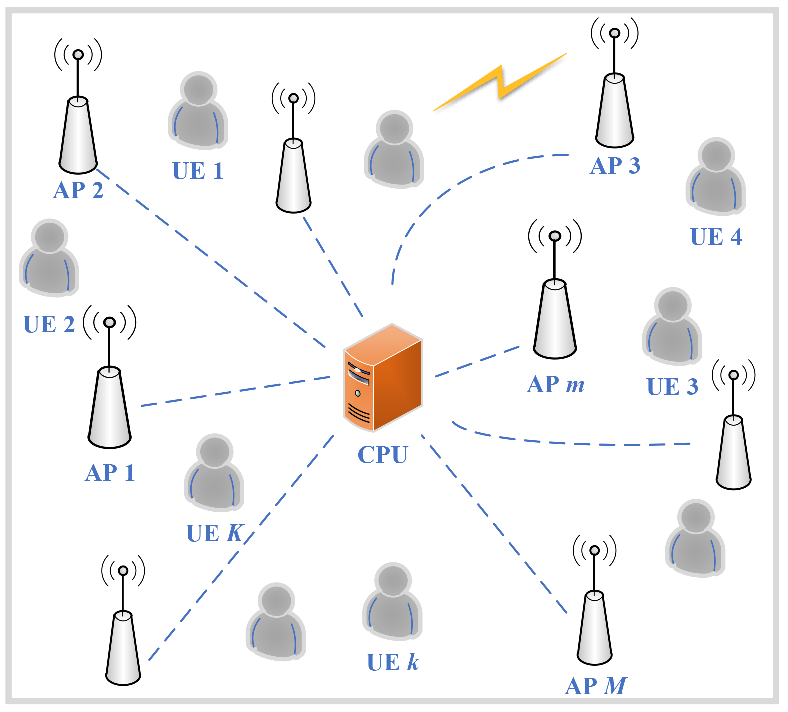
\includegraphics[width=2.9in] {fig1}
\caption{System model of CF-mMIMO with nonlinear PAs and low-resolution ADCs.}
\label{fig1}
\end{figure}

\section{System Model}
In this paper, we consider an uplink CF-mMIMO system as shown in Fig. \ref{fig1}, which consists of $M$ $N$-antenna APs and $K$ single-antenna UEs. All APs are connected to the central processing unit (CPU) through backhaul links. The system employs a time-division duplex (TDD) protocol for data transmission. Since this paper only focuses on the uplink data transmission phase, the coherence time interval is divided into two stages: uplink training and uplink data transmission. 

\subsection{Channel Estimation}
In this study, we adopt an uncorrelated Rayleigh fading channel model \cite{paperIA11}. The channel gain between the $m$-th AP and the $k$-th UE is denoted as 
\begin{equation}\mathbf{g} _{mk} = {\beta _{mk}^{1/2} } {{\bf{h}}_{mk}},\end{equation}
which takes into account both large-scale fading effects $\beta  _{mk}$ and small-scale fading $\mathbf{h} _{mk}$. Among them, $\beta_{mk}$ considers both geometric attenuation and shadow fading simultaneously, and it is assumed to remain constant within a coherence time interval. The elements of $\mathbf{h}_{mk}$ are complex Gaussian random variables with Rayleigh-distributed envelopes. Let $\tau_\text{c}$ be the length of the coherence interval and $\tau_\text{p}$ represents the uplink training time for each coherence interval. Due to the length limitation of training time, we employ non-orthogonal pilots with $\tau_\text{p} < K$ and define the set $\mathcal{P}_k$ of UEs that utilize the identical pilot sequence as the $k$-th UE. During the uplink training phase, all $K$ users simultaneously send non-orthogonal pilot sequences to all APs. The pilot signal of the $k$-th UE can be expressed as $\sqrt{\tau_\text{p}}\boldsymbol{\varphi}_k\in \mathbb{C} ^{\tau_\text{p}\times1}$ with $\left\|\boldsymbol{\varphi}_k\right\|^2=1$. 

In this paper, we employ a more refined deterministic behavioral model of hardware nonlinearities, aiming to model the main factors contributing to hardware impairments more accurately \cite{paper1}. One of the main advantages of this deterministic behavioral model is that it can characterize the physical effects of various hardware damages using a small number of parameters. It describes the hardware input-output relationship as \cite{paper2}
\begin{equation}
x_\text{out}=\sum_{i=0}^{N_p}a_{2i+1}x_\text{in}\left | x_\text{in} \right |^{2i}  
\end{equation}
where $a_{2i+1}$ are the model complex coefficients, and the nonlinearity degree can be expressed as $2N_p + 1$. The model collectively accounts for the nonlinearities of amplifiers, local oscillators, mixers, and other hardware components. It is important to note that, for in-band distortion, only odd-order terms are present in the quasi-memoryless polynomial due to the occurrence of even-order terms outside the band. Furthermore, the third-order term captures the primary sources of nonlinearity in radio frequency amplifiers \cite{paper3}, \cite{paper4}. Consequently, we adopt the third-degree polynomial model with $N_p=1$. There are results indicating that the third-order polynomial model has good accuracy and can effectively approximate the actual nonlinear behavior of PAs \cite{paper5}, \cite{paper6}. After the nonlinear behavior of PAs, the output signal of the $k$-th UE is denoted as 
\begin{equation}\label{eqn-1}\boldsymbol{\phi }_k = \underset{\tilde{a}_1 }{\underbrace{{a_1}\sqrt {{\tau _\text{p}}}} }  \boldsymbol{\varphi }_k + \underset{\tilde{a}_3 }{\underbrace{{a_3}{\tau _\text{p}}\sqrt {{\tau _\text{p}}}} }  \boldsymbol{\varphi} _k{\left\| {\boldsymbol{\varphi }_k} \right\|^2},\end{equation}
where $\tilde{a}_1 \triangleq a_1\sqrt{\tau_\text{p}} $, $\tilde{a}_3 \triangleq a_3\tau_\text{p}\sqrt{\tau_\text{p}} $. The pilot matrix received by the $m$-th AP is
\begin{equation}\label{eqn-2}
\begin{aligned}
\mathbf{Y}_{\text{p},m} &= \sqrt {{\rho _\text{p}}}\sum_{k=1}^{K}  {{\bf{g}}_{mk}}\boldsymbol{\phi }_k^H + {\mathbf{W}_{\text{p},m}} \\
&= \sqrt {{\rho _\text{p}}}\sum_{k=1}^{K}  ({\tilde{a}_1}{{\bf{g}}_{mk}}\boldsymbol{\varphi} _k^H + \tilde{a}_3 {{\bf{g}}_{mk}}\boldsymbol{\varphi} _k^H{\left\| {\boldsymbol{\varphi }_k} \right\|^2}) + {\mathbf{W}_{\text{p},m}},
\end{aligned}
\end{equation}
where ${\rho _\text{p}}$ is the normalized signal-to-noise ratio (SNR) for pilot signals. Besides, ${\mathbf{W}_{\text{p},m}} \in \mathbb{C}  {^{N \times {\tau _\text{p}}}}$ denotes the additive white Gaussian noise (AWGN) matrix at the $m$-th AP with the $\varsigma-$th column distributed
as $\left [ \mathbf{W}_{\text{p},m} \right ] _\varsigma \sim \mathcal{CN} (\mathbf{0},\mathbf{I}_N)$. 

We utilize a non-uniform quantizer to investigate the impact of low-resolution ADCs on the system. To this end, we adopt the well-known additive quantization noise model (AQNM), which describes the distortion introduced by the quantization process as a Gaussian random variable. The model has been demonstrated to be sufficiently accurate under conditions of low-medium-SNR \cite{paper7}, \cite{paper8}. With \eqref{eqn-2}, the output of the ADC at the $m$-th AP is given by
\begin{align}\label{eqn-3}{\tilde {\bf{Y}}_{\text{p},m}} & \triangleq {\alpha _m}{\mathbf{Y}_{\text{p},m}} + {\tilde {\bf{W}}_{\text{p},m}} \nonumber\\
&= {\alpha _m}\sqrt {{\rho _\text{p}}} \sum_{k=1}^{K}  ({\tilde{a} _1}{{\bf{g}}_{mk}}\boldsymbol{\varphi} _k^H + {\tilde{a}_3}{{\bf{g}}_{mk}}\boldsymbol{\varphi} _k^H{\left\| {\boldsymbol{\varphi}_k} \right\|^2}) \nonumber \\
&\quad+ {\alpha _m}{\mathbf{W}_{\text{p},m}} + {\tilde{\bf{W}}_{\text{p},m}},\end{align}
where the associated parameter ${\alpha_m}$ dictates the accuracy of the ADC at the $m$-th AP and is determined by the number of quantization bits $b_m$ \cite{paper9}. Besides, ${\tilde{\mathbf{W}}_ {\text{p}, m}}$ in \eqref{eqn-3} represents the additive Gaussian quantization noise at the $m$-th AP, which is uncorrelated with $\mathbf{Y}_{\text{p},m}$ and its covariance matrix can be expressed as
\begin{align}\label{eqn-4}
\mathbf{R}_{\tilde{ \mathbf{W}}_{\text{p},m}} &= \mathbb{E}\left\{ {{\tilde{\mathbf{W}}_{\text{p},m}}\tilde {\mathbf{W}}_{\text{p},m}^H} \right\} \nonumber\\ 
&= {\alpha _m}(1 - {\alpha _m})\text{diag}\left(\mathbb{E}\left\{ {{\mathbf{Y}_{\text{p},m}}\mathbf{Y}_{\text{p},m}^H} \right\} \right). 
\end{align}

Once the received pilot signal at the $m$-th AP has been quantized, projecting the quantized signal $\tilde {\mathbf{Y}}_{\text{p},m}$ onto $\boldsymbol{\varphi}_k$ can yield
\begin{align}\label{eqn-5}
\check{\mathbf{y} }_{\text{p},mk}&\triangleq {\tilde{\mathbf{Y}}_{\text{p},m}}\boldsymbol{\varphi }_k \nonumber\\
%&= {\alpha _m}\sqrt {{\rho _p}} \mathop \sum \nolimits_{k' = 1}^K ({b_1}{{\bf{g}}_{mk'}}\varphi _{k'}^H + {b_3}{{\bf{g}}_{mk'}}\varphi _{k'}^H{\left| {{\varphi _{k'}}} \right|^2}){\varphi _k} + {\alpha _m}{W_{p,m}}{\varphi _k} + {{\tilde W}_{p,m}}{\varphi _k}\\
&= {\alpha _m}\sqrt {{\rho _\text{p}}}\sum_{k'\in \mathcal{P}_k }^{K}  ({\tilde{a}_1} + {\tilde{a}_3}\tau_\text{p}){{\bf{g}}_{mk}}\nonumber \\
&\quad + {\alpha _m}{\mathbf{W}_{\text{p},m}}\boldsymbol{\varphi}_k + {{\tilde{\mathbf{W}}}_{\text{p},m}}\boldsymbol{\varphi}_k.
\end{align}
Based on the above calculations, we have the following lemma.

\textit{Lemma:}
The channel estimation of ${{\bf{g}}_{mk}}$, obtained through the application of the minimum mean square error (MMSE) method, can be expressed as 
\begin{equation}\label{eqn-6}
\mathbf{\hat{g} }_{mk} = c_{mk} \mathbf{\check{y} }_{\text{p},mk},
\end{equation}
where 
\begin{align}\label{eqn-7}
{c_{mk}} &= \mathbb{E}\left \{ \mathbf{g}_{mk}^H\mathbf{\check{y} }_{\text{p},mk}   \right \} \left ( \mathbb{E}\left \{  \mathbf{\check{y} }_{\text{p},mk}^H\mathbf{\check{y} }_{\text{p},mk}\right \}   \right )^{-1}   \nonumber \\
%&= \frac{{\sqrt {{\tau _p}{\rho _p}} N{\beta _{mk}}{\alpha _m}({a_1} + {a_3}{\tau _p})}}{{N{\alpha _m}({\tau _p}{\rho _p}({a_1} + {a_3}{\tau _p}){\beta _{mk}} + 1)}}{{\bf{\mathord{\buildrel{\lower3pt\hbox{$\scriptscriptstyle\smile$}} \over y} }}_{p,mk}} \\%
&= \frac{{\sqrt {{\tau _\text{p}}{\rho _\text{p}}} {\beta _{mk}}({a _1} + {a _3}{\tau _\text{p}})}}{{{\tau _\text{p}}{\rho _\text{p}}\sum_{k'\in \mathcal{P}_k }^{K} ({a _1} + {a _3}{\tau _\text{p}})^2{\beta _{mk}} + 1}}.
\end{align}

The mean-square of the $n$-th component of channel estimation is denoted as
\begin{align}\label{eqn-8}
\gamma_{m k}&=\mathbb{E}\left \{ \left | \left [ \mathbf{\hat{g} }_{mk}  \right ]_n  \right |^2  \right \}\nonumber \\ &=\frac{\tau_\text{p} \rho_\text{p} \alpha_{m} \beta_{m k}^{2}\left(a_{1}+a_{3} \tau_\text{p}\right)^{2}}{\tau_\text{p} \rho_\text{p}\sum_{k'\in \mathcal{P}_k }^{K} \left(a_{1}+a_{3} \tau_\text{p}\right)^2 \beta_{m k}+1}.
\end{align}

Let ${{\bf{\tilde g}}_{mk}} = {{\bf{g}}_{mk}} - {{\bf{\hat g}}_{mk}}$ denote the channel estimation error. According to the properties of linear MMSE estimation, ${{\bf{\tilde g}}_{mk}}$ and ${{\bf{\hat g}}_{mk}}$ are independently complex Gaussian distributed. Consequently, the mean-squared error of the channel estimation for the elements of ${{\bf{\tilde g}}_{mk}}$ satisfies $\left [ {{\bf{\tilde g}}_{mk}} \right ]_n\sim \mathcal{CN} \left ( 0, \left ( \beta _{mk}-\gamma _{mk} \right ) \right ) $.
\subsection{Uplink Data Transmission}
During the uplink data transmission phase, all UEs simultaneously send their data ${q_k}$ to the APs, where $\mathbb{E}  \left \{ \left | q_k \right |^2  \right \} =1, \forall k$. After the nonlinear behavior of the PA on the UE side, the output signal of the $k$-th UE is
\begin{align}
\label{eqn-9}{y_k} &= \sqrt {{\rho _\text{u}}} \left( {{a_1}\sqrt {{\eta _k}} {q_k} + {a_3}\sqrt {{\eta _k}} {q_k}{{\left| {\sqrt {{\eta _k}} {q_k}} \right|}^2}} \right)\nonumber \\ 
&= \sqrt {{\rho _\text{u}}} \left( {{\tilde{a}_{1k}}{q_k} + {\tilde{a}_{3k}}{q_k}{{\left| {{q_k}} \right|}^2}} \right),
\end{align}
where $\rho _\text{u}$ denotes the maximum normalized transmit power at each UE, $\tilde{a}_{1k} \triangleq a_1\sqrt{\eta _k}$, and $\tilde{a}_{3k} \triangleq a_3\eta _k\sqrt{\eta _k}$. Besides, the power control coefficients $\eta _k, \forall k$ are chosen to satisfy $\mathbb{E}\left\{ {{{\left| {{y_k}} \right|}^2}} \right\} \le {\rho _\text{u}}$. Thus, the constraint can be simplified as
\begin{equation}\label{eqn-10}
{\left| {{a_1}} \right|^2}{\eta _k} + 2(a_1^ * {a_3} + {a_1}a_3^ * )\eta _k^2 + 6{\left| {{a_3}} \right|^2}\eta _k^3 \le 1,  \forall k.
\end{equation}

The complex baseband signal received at the $m$-th AP can be expressed as
\begin{equation}\label{eqn-11}
{{\bf{y}}_{\text{u},m}} = \sqrt {{\rho _\text{u}}} \sum_{k = 1}^K ({\tilde{a}_{1k}}{{\bf{g}}_{mk}}{q_k} + {\tilde{a}_{3k}}{{\bf{g}}_{mk}}{q_k}{\left| {{q_k}} \right|^2}) + {\bf{w}}_{\text{u},m},
\end{equation}
where $\mathbf{w}_{\text{u},m}\sim \mathcal{CN} (\mathbf{0},\mathbf{I}_N) $ denotes the additive noise. Subsequently, the signal received by the $m$-th AP is quantized by the ADCs. The output of this process is expressed as
\begin{align}\label{eqn-12}{{\bf{\tilde y}}_{\text{u},m}} &= {\alpha _m}{{\bf{y}}_{\text{u},m}} + {{\bf{\tilde w}}_{\text{u},m}} \nonumber\\
&= {\alpha _m}\sqrt {{\rho _\text{u}}} \sum_{k = 1}^K ({\tilde{a}_{1k}}{{\bf{g}}_{mk}}{q_k} + {\tilde{a}_{3k}}{{\bf{g}}_{mk}}{q_k}{\left| {{q_k}} \right|^2}) \nonumber\\
&\quad+ {\alpha _m}{{\bf{w}}_{\text{u},m}} + {{\bf{\tilde w}}_{\text{u},m}},
\end{align}
where ${{\bf{\tilde w}}_{\text{u},m}}$ denotes the quantization noise, and its convariance matrix can be given as 
\begin{align}{\mathbf{R}_{{{{\bf{\tilde w}}}_{\text{u},m}}}} \approx {\alpha _m}(1 - {\alpha _m})\text{diag}(\mathbb{E}\left\{ {{{\bf{y}}_{\text{u},m}}{\bf{y}}_{\text{u},m}^H} \right\}).\end{align}

To detect $q_k$, each AP employs a distributed approach to compute local data estimations through low-complexity matched filtering combining. The signals are then forwarded to the CPU for aggregation and decoding through the fronthaul link. Therefore, the received signals at the CPU can be expressed as
\begin{align}\label{eqn-14}
{r_{\text{u},k}} &= \sum_{m = 1}^M {\bf{\hat{g}}}_{mk}^H{{{\bf{\tilde y}}}_{\text{u},m}}\nonumber\\
& = \sqrt {{\rho _\text{u}}}  \sum_{m = 1}^M {\alpha _m}\sum_{k' = 1}^K {\bf{\hat g}}_{mk}^H{\tilde{a}_{1k'}}{{\bf{g}}_{mk'}}q_{k'}  
\nonumber\\& \quad+ \sqrt {{\rho _\text{u}}} \sum_{m = 1}^M {\alpha _m}\sum_{k' = 1}^K {\bf{\hat g}}_{mk}^H{\tilde{a}_{3k'}}{{\bf{g}}_{mk'}}q_{k'} {\left| {q_{k'} } \right|^2}
 \nonumber\\& \quad+ \sum_{m = 1}^M {\bf{\hat g}}_{mk}^H{\alpha _m}{{\bf{w}}_{\text{u},m}} + \sum_{m = 1}^M {{{\bf{\hat g}}}^H_{mk}}{{{\bf{\tilde w}}}_{\text{u},m}}.
\end{align}

Subsequently, $q_k$ is detected from $r_{\text{u},k}$. In the following section, we will derive a closed-form expression for the achievable rate.

\subsection{Achievable rate Analysis}
In this part, we derive the achievable rate of the uplink UEs in CF-mMIMO systems while taking into account the nonlinear behavior of PAs and low-resolution ADCs. Based on this fact, the CPU is unable to access the actual channel state because the AP only has channel estimation information. Although the CPU is unknown to the current actual channel states, it assumes that the average value of the channel states is known and utilizes this known average value to calculate the achievable rate \cite{paper6}. With \eqref{eqn-14}, the signal received at the CPU can be reformulated as
\begin{align}\label{eqn-15}
{r_{\text{u},k}}& = {\text{ES}_k} \cdot {q_k} + {\text{BU}_k} \cdot {q_k} + \sum_{k' \ne k}^K {\text{I}_{kk'}} \cdot q_{k^\prime} \nonumber \\
&\quad+\sum_{k' \ne k}^K {\text{NB}_{kk'}} \cdot q_{k^\prime}  + {\text{N}_k} + {\text{Q}_k},
\end{align}
where ${\text{ES}_k}$, ${\text{BU}_k}$, ${\text{I}_{kk'}}$, ${\text{NB}_{kk'}}$, ${\text{N}_k}$, and ${\text{Q}_k}$ respectively represent the deterministic value of the desired signal of the $k$-th UE, the uncertainty of beamforming, the interference caused by the $k'$-th UE, the interference from nonlinear PAs in the $k$-th UE, the additive noise, and the quantization noise, which can be specifically expressed as
\begin{equation}\label{eqn-16}
{\text{ES}_k} = \sqrt {{\rho _\text{u}}} \mathbb{E}\left\{ {\sum_{m = 1}^M {\alpha _m}\left({\tilde{a} _{1k}}{\bf{\hat g}}_{mk}^H{{\bf{g}}_{mk}} + {\tilde{a} _{3k}}{\bf{\hat g}}_{mk}^H{{\bf{g}}_{mk}}{{\left| {{q_k}} \right|}^2}\right)} \right\},
\end{equation}
\begin{equation}\label{eqn-17}
\begin{aligned}{\text{BU}_k} &= \sum_{m = 1}^M \alpha_m \sqrt{\rho _\text{u}}\left({\tilde{a} _{1k}}{\bf{\hat g}}_{mk}^H{{\bf{g}}_{mk}} + {\tilde{a} _{3k}}{\bf{\hat g}}_{mk}^H{{\bf{g}}_{mk}}{\left| {{q_k}} \right|^2}\right)\\ 
&- \mathbb{E} \left\{ {\sum_{m = 1}^M {\alpha _m}\sqrt{\rho _\text{u}}\left({\tilde{a} _{1k}}{\bf{\hat g}}_{mk}^H{{\bf{g}}_{mk}} + {\tilde{a} _{3k}}{\bf{\hat g}}_{mk}^H{{\bf{g}}_{mk}}{{\left| {{q_k}} \right|}^2}\right)} \right\},
\end{aligned}\end{equation}
\begin{equation}\label{eqn-18}{\text{I}_{kk'}} = \sqrt {{\rho _\text{u}}}\sum_{m = 1}^M {\alpha _m}{\tilde{a}_{1k'}}{{\bf{\hat g}}^H_{mk}}{{\bf{g}}_{mk'}},\end{equation}
\begin{equation}\label{eqn-19}{\text{NB}_{kk'}} = \sqrt {{\rho _\text{u}}} \sum_{m = 1}^M {\alpha _m}{\tilde{a}_{3k'}}{{\bf{\hat g}}^H_{mk}}{{\bf{g}}_{mk'}}{\left| {{q_{k'}}} \right|^2},\end{equation}
\begin{equation}\label{eqn-20}{\text{N}_k} = \sum_{m = 1}^M {\alpha _m}{\bf{\hat g}}_{mk}^H{{\bf{w}}_{\text{u},m}},\end{equation}
\begin{equation}\label{eqn-21}{\text{Q}_k} = \sum_{m = 1}^M {{\bf{\hat g}}^H_{mk}}{{\bf{\tilde w}}_{\text{u},m}}.\end{equation}

We treat the sum of interference and noise in \eqref{eqn-15} as effective noise. Therefore, by considering the interference term as a random variable of uncorrelated Gaussian noise in the worst case, we can obtain the achievable uplink rate for the $k$-th user as \eqref{eqn-22}, shown at the top of the next page.

\textit{Theorem 1}: In the CF-mMIMO system with CB, for any finite $M$ and $K$, the achievable rate for the $k$-th UE is given by  \eqref{eqn-23}, shown at the top of the next page.

\textit{Proof}: See Appendix.

\begin{figure*}[ht]
	\centering
	\begin{equation}\label{eqn-22}
		{R_{\text{u},k}}= {\log _2}\left(1 + \frac{{{{\left| {{\text{ES}_k}} \right|}^2}}}{{\mathbb{E}\left \{\left |  \text{BU}_k \right | ^2 \right \}   +\sum \limits_{k'\ne k}^{K} \mathbb{E} \left \{ \left | \text{I}_{kk'} \right |^2  \right \}   +  \sum \limits_{k'\ne k}^{K}\mathbb{E}\left \{ \left |  {\text{NB}_{kk'}}  \right |^2  \right \}  +\mathbb{E} \left \{ \left | {\text{N}_k} \right |^2  \right \}   +  \mathbb{E}\left \{ \left |  \text{Q}_k\right | ^2 \right \}  } }\right).
	\end{equation}
	\hrulefill
	\begin{equation}\label{eqn-23}
		R_{\text{u}, k}=\log _{2}\left(1+\frac{N^{2} \rho_\text{u}\left|\tilde{a}_{1 k}+\tilde{a}_{3 k}\right|^{2}\left(\sum\limits_{m=1}^{M} \alpha_{m} \gamma_{m k}\right)^{2}}{N^{2} \rho_\text{u} \sum\limits_{k'=1}^{K}\left(\Omega_{k^{\prime}} \sum\limits_{m=1}^{M} \alpha_{m}^{2} \gamma_{m k} \beta_{m k'}\right)+3 N^{2} \rho_\text{u}\left|a_{3}\right|^{2} \eta_{k}^{3}\left(\sum\limits_{m=1}^{M} \alpha_{m}^{2} \gamma_{m k}\right)^{2}+N^{2} \sum\limits_{m=1}^{M} \alpha_{m}^{2} \gamma_{m k}+\Psi _k }\right),
	\end{equation}
	\flushleft{where}
	\begin{equation}\begin{aligned}\Omega _k = \left( {{{\left| {{a_1}} \right|}^2}{\eta _{k}} + 2a_1^*{a_3}{\eta _{k}^2}+ 2{a_1}a_3^ * \eta _{k}^2 + 6{{\left| {{a_3}} \right|}^2}\eta _{k}^3} \right), \end{aligned}\end{equation}
	\begin{equation}\Psi _k={N}{\rho _\text{u}}\mathop \sum \limits_{m = 1}^M {\alpha _m}(1 - {\alpha _m})\left( {\mathop \sum \limits_{k = 1}^K {\beta _{mk}}\Omega _k + 1} \right){\gamma _{mk}}.\end{equation}
	\hrulefill
\end{figure*}

Based on \eqref{eqn-23}, we provide some insights into the performance of CF-mMIMO systems equipped with nonlinear PAs and low-resolution ADCs.

Theorem 1 derives an exact closed-form expression for the achievable rate, which clearly reveals the intrinsic correlation between key parameters and system performance. Specifically, the coefficient $a_3$ in \eqref{eqn-23} represents the nonlinear behavior of PAs. With the enhancement of PA nonlinear behavior, the absolute value of $a_3$ shows an increasing trend. This change leads to a decrease in the numerator and an increase in the denominator of the SINR, resulting in a sharp decrease in the user rate. It indicates that the nonlinear behavior of the PA has a significant negative impact on the user rate.
In addition, from the composition of the numerator and denominator of the expression, all terms except the quantization noise term contain the square factor of $N$. After dividing the numerator and denominator by the square of $N$, we find that only the term of ${\rho _\text{u}}\mathop \sum \limits_{m = 1}^M {\alpha _m}(1 - {\alpha _m})\left( {\mathop \sum \limits_{k = 1}^K {\beta _{mk}}\Omega _k + 1} \right){\gamma _{mk}}/N$ contains $N$ elements. As $N$ gradually increases, there is a certain degree of increase in the initial user rate. When $N$ is sufficiently large relative to ${\rho _\text{u}}\mathop \sum \limits_{m = 1}^M {\alpha _m}(1 - {\alpha _m})\left( {\mathop \sum \limits_{k = 1}^K {\beta _{mk}}\Omega _k + 1} \right){\gamma _{mk}}$, its impact on the rate tends to be close to zero.

\section{Uplink Sum-Rate Maximization}
As a consequence of the APs receiving signals from all UEs, the rate of the target user can be significantly degraded by inter-user interference. It is essential to regulate the transmission power of other users to manage the relationship between the target signal and the interference signals.

Based on the above background and the adjustable variable parameters in the closed-form solution, this section constructs an uplink power control model. Grounded in the set of non-negative powers, the model aims to maximize the sum rate of the system. The optimization process adheres to the system's power constraint conditions, that is, each variable does not exceed the pre-set maximum power limit. In accordance with equation \eqref{eqn-23}, the uplink sum-rate maximization problem is mathematically expressed as
\begin{align} \label{P1}
\mathcal{P}_1:& \quad \underset{\left \{ \eta _k \right \} }{\text{max}} \quad  {\sum_{k=1}^{K}} R_{\text{u},k}\\
\text{s.t.}&\quad {\left| {{a_1}} \right|^2}{\eta _k} + 2(a_1^ * {a_3} + {a_1}a_3^ * )\eta _k^2 + 6{\left| {{a_3}} \right|^2}\eta _k^3 \le 1, \forall k.
\end{align}

In general, $\mathcal{P}_1$ behaves as a non-convex NP-hard problem. Its characteristics make it impossible for model-based approaches to accurately quantify the performance gap with respect to the optimal solution and also lead to high computational complexity \cite{paper6}. Moreover, the adaptability of model-based methods is constrained, exhibiting difficulties in accommodating the diversity of future heterogeneous service demands and stochastic variations in the environment in a flexible manner. It is noteworthy that the CSI $\mathbf{g} _{mk}$ is regarded as a crucial statistic in solving this problem, as it encodes vital information for identifying optimal power control schemes \cite{paperIA17}. Consequently, there exists a potential functional relationship capable of mapping $\mathbf{g}_{mk}$ onto corresponding power control coefficients $\eta_k$. In light of these challenges, we will adopt a data-driven DRL algorithm to explore and realize this mapping function.

Furthermore, based on the formulation in equation \eqref{eqn-23}, we deduce that the user rate monotonically increases with the ADC resolution $\alpha_m$. Taking into account the quantization noise term, we can dynamically adjust the number of bits in the ADC resolution to maximize the sum rate. To this end, we will employ an improved deep Q-learning algorithm as an optimization tool. With the target of maximizing the user sum rate, the ADC resolution allocation problem is formally stated as
\begin{align}\label{P2}
\mathcal{P}_2 :&\quad\underset{\left \{ b_m \right \} }{\text{max}} \quad  {\sum_{k=1}^{K}} R_{\text{u},k}\\
\text{s.t.}&\quad   b_m=0,1,2,...,  \forall m, \\
\quad & \quad N\sum_{m=1}^{M} b_m=B_\text{\text{max}},
\end{align}
where $B_\text{max}$ is the fixed total resolution bit for all ADCs on the APs.

Based on the above two optimization problems, we employ two algorithms in the following two sections to explore the performance of the CF-mMIMO system.

\section{Design Of DMAGNN-AC Algorithm}

In deep reinforcement learning, the Markov decision process (MDP) is a core concept for modeling sequential decision-making problems. Typically, in an MDP problem, there are usually one or more agents interacting with the environment. The agent picks and executes an action $a$ based on a policy function $\pi$ and the current state $s$. The environment provides feedback in the form of a reward $r$ to evaluate the goodness of the action $a$ and transitions to the next state $s'$. In a complete episode, the agent makes several such action choices, and these actions and state transitions together form an MDP characterized by the tuple $(\mathcal{S},\mathcal{A} ,\mathcal{P} ,\mathcal{R}   )$. Among them, $\mathcal{S}$ denotes the state space, $\mathcal{A}$ represents the action space. Additionally, $\mathcal{P}$ signifies the state transition probability function, which refers to the probability of transitioning to state $s'$ after executing action $a$ in state $s$. Lastly, $\mathcal{R}$ designates the reward function, which defines the expected return after executing action $a$ in state $s$.

We model the optimization problem $\mathcal{P}_1$ as an MDP problem in order to implement power allocation by using DRL algorithm. However, due to the complex interference relationships and spatial correlations between UEs, DRL is difficult to effectively learn the optimal strategy \cite{paper11}. To address this issue, we design a DMAGNN framework to extract the interference features of UE, which provides structured state information and can effectively improve the performance of DRL. In this framework, the CPU serves as an agent, while the environment consists of components such as UEs and APs. The proposed DMAGNN models the CSI between UEs and APs as node features and models the interference between different UEs as edges. The detailed setup and specific process description of the neural network are shown in Fig. \ref{fig2}, located at the top of this page.

\begin{figure}
\centering

\includegraphics[width=3.6in] {fig2}
\caption{Network architecture of DMAGNN-AC.}
\label{fig2}
\end{figure}

\subsection{DMAGNN-AC  Components}

$\emph{1) State}$: In Section III, we mentioned the existence of a function that maps the CSI $\mathbf{g}_{mk}$ between the $k$-th UE and the $m$-th AP to the power control coefficient $\eta_k$ of the $k$-th UE. However, due to the fact that CPU lack channel realizations, we ultimately decided to use the theoretical CSI $\mathbf{g}_{mk}$ as the input to the neural network. Thus the input to the neural network can be expressed as
\begin{equation}\mathbf{\Gamma}^t:=\left \{  \mathbf{g}_{mk}^t  \mid \forall m,k\right \}.	\end{equation} 

However, considering that the training process is essentially a Markov process closely related to time series, it is not desirable to directly use the variable $\mathbf{\Gamma}^t$ as an input to the neural network. Concurrently, the changes in environmental states triggered by user movement behavior within a designated time span can be conceptualized as a time-series evolutionary process. In this evolutionary process, the characteristics of user mobility in the temporal and spatial dimensions serve as pivotal guides for predicting their actions in the subsequent moments. 
Therefore, we introduce $\mathbf{g}_{mk}$ and $R_{\text{u},k}$ at the moment $(t-1)$ as auxiliary information for the input to the neural network, so that they can participate in the prediction of the action at the next moment together with $\mathbf{\Gamma}^t$. The specific definition of auxiliary information is 
\begin{equation}\mathbf{\Xi} ^{t-1}:=\left \{\mathbf{g}_{mk}^{t-1} , R_{\text{u},k}^{t-1} \mid \forall m,k \right \}  .\end{equation} 

The final input of a neural network can be represented as
\begin{equation}s^{t}:=\left \{ \mathbf{\Xi} ^{t-1}, \mathbf{\Gamma} ^t\right \}. \end{equation}

At this point, the cardinality of the state is $2 \left ( MK \right ) +K$.


$\emph{2) Action}$:
The actor network makes decisions based on the current state $s$ and outputs the uplink transmission power coefficients for $K$ UEs, expressed as
\begin{equation}a ^{t}=\left [ \eta _1^{t},...,\eta _K^{t} \right ] ,\end{equation}
where $0\le \eta _k^{t}\le \eta _\text{max}, \forall k$.

\emph{3) Reward}: We directly use the implemented user rate to represent the rewards for environmental feedback, which is defined as
\begin{equation}r^{t+1} = \textstyle \sum_{k=1}^{K} R_{\text{u},k}^{t}.\end{equation}

\subsection{Proposed Algorithm Design}
The specific design of the proposed algorithm is reflected in the following four aspects.

\subsubsection{Actor Network Layered Design}
The actor network is designed with a layered structure, aiming to reasonably divide the functions and effectively integrate the information. Specifically, the upper network primarily extracts and integrates the features of information $\mathbf{\Xi }^{t-1} $. Subsequently, the output of the upper layer network is combined with the features of information $\mathbf{\Gamma} ^t$ as the input to the lower layer network. The main function of the lower layer network is to perform action prediction based on the features mentioned above. 

Before inputting $\mathbf{\Gamma} ^t$ into the lower layer network, we use our independently developed DMAGNN to extract features from $\mathbf{\Gamma} ^t $. The operation process of DMAGNN includes the following steps:
\begin{itemize}
\item {\bf{Node feature initialization:}}
The node characteristics of the $k$-th UE at time $t$ are initialized as
\begin{equation}\label{eq-38}x_k=\text{vec}(H_{\text{in},k}^HH_{\text{in},k})\in \mathbb{R}^d, \end{equation}
where $H_{\text{in},k}\in \mathbb{C} ^{M\times N}$ is the channel matrix from the $k$-th UE to $M$ APs.

\item{\bf{Dynamic Graph Structure Learning:}}
In constructing the graph, we consider that the traditional graph structure relies on fixed geographic distances (e.g., path loss) to define connectivity \cite{paper11}, \cite{paper12}. However, in CF-mMIMO systems, the UE distribution is dense and the interference patterns are complex. Fixed graphs cannot reflect the influence of instantaneous channel states \cite{paper10}. Therefore, we draw on the attention mechanism of graph attention networks (GAT) to introduce a learnable parameterized distance metric \cite{paper13}. The strength of the association between nodes $i$ and $j$ is calculated using a bilinear attention mechanism
\begin{equation}\label{eq-39}a_{ij}=\sigma \left ( \frac{\left ( W_qx_i \right ) \cdot \left ( W_kx_j \right )  ^T}{\sqrt{b} } \right  ), \end{equation}
where $b $ is the scaling factor, $W_q$ and $W_k$ are trainable projection matrices that map node features $x_i$, $x_j$ to query and key spaces. The query space is used to represent the ‘query’ features of the current node (e.g., UE $i$), while the key space is used to represent the ‘queried’ features of other nodes (e.g., UE $j$). By calculating the dot product of them, the correlation and similarity between the two nodes can be measured. This mechanism allows this model to dynamically learn relationships between nodes rather than relying on a predefined graph structure.

{\emph{Theorem 2:}} To reduce the computational complexity $O(K^2)$ of fully connected graphs, we design a sparse adjacency matrix form
\begin{equation}\label{eq-40}A_{ij}=\left\{\begin{matrix}
  1,& \text{if} \hspace{0.1cm} a_{ij}> \vartheta \hspace{0.1cm} \text{and}\hspace{0.1cm} i\ne j\\ 
  0,& \text{otherwise},
\end{matrix}\right.\end{equation}
where the dynamic threshold $\vartheta$ is determined by an adaptive binary search to ensure that the number of non-zero edges satisfies $\left | E \right | =O\left ( K\log_{}{K}  \right ) $. Adjacency matrix sparsification only retains relatively strongly correlated connections, which improves the generalization of the model.

\item{\bf{Multi-scale feature aggregation:}}
Multi-scale convolution aggregates neighbor information from different ranges to enhance the model's ability to capture complex spatial correlations \cite{paper14}, which solves the problem of limited receptive field in traditional single-layer graph convolutional networks (GCN). The multi-hop information aggregation formula is expressed as
\begin{equation}\label{eq-41}\text{GCN}\left ( A,H_{\text{in}} \right ) =\sum_{l=0}^{L} \tilde{A} ^lH_{\text{in}}W_l,\end{equation}
where $\tilde{A} =D^{-\frac{1}{2} }AD^{-\frac{1}{2} }$ denotes the symmetric normalization of $A$, $D=\text{diag}\left (  {\textstyle \sum_{j}^{}A_{1j},..., {\textstyle \sum_{j}^{}A_{Kj}} }  \right ) $ indicates the degree matrix, and $W_l\in \mathbb{R}^{d\times d} $ represents the trainable weight matrix for the $l$-th hop. This design meets the following characteristics:
\begin{itemize}
    \item Locality preservation: $l=0$ preserves the characteristics of the node itself.
    \item Neighborhood expansion: $l=1$ aggregates first-order neighbor information, while $l=2$ captures second-order neighbor information.
\end{itemize}
Meanwhile, independent $W_l$ are used for different hops to avoid feature confusion.

\item{\bf{Gate control feature update mechanism:}}
Finally, we adopt gating mechanism to assist the model in selectively updating node features. The specific process can be expressed as
\begin{equation}\label{eq-42}Z=\text{GCN}\left ( A,H_{\text{in}} \right ), \end{equation}
\begin{equation}\label{eq-43}G=\sigma \left ( W_g\left [ H_{\text{in}}  \oplus Z \right ]  \right ),\end{equation}
\begin{equation}\label{eq-44}H_{\text{out}}=\text{LayerNorm}\left ( G\odot H_{\text{in}}+\left ( 1-G \right ) \odot Z \right ), \end{equation}
where $Z$ is the new feature generated after convolution and $W_g\in \mathbb{R}^{2d\times d}$ represents the gating weight matrix. The gating mechanism can dynamically select how many original features ($H_{\text{in}}$) and new features ($Z$) to retain, thereby alleviating the problem of gradient vanishing.
\end{itemize}

\begin{algorithm}[t]
    \renewcommand{\algorithmicrequire}{\textbf{Input:}}
    \renewcommand{\algorithmicensure}{\textbf{Output:}}
    \caption{DMAGNN-AC Power Allocation Algorithm}
    \label{DDPG}
    \begin{algorithmic}[1]
    			\State $\emph{Input:}$ Episode times $T_e$, exploration times $T$, discount factor $\gamma$, learning rate $\alpha$, random data quantity $R_q$, batch size $\mathcal{N}$, and neural network updating weights $\tau$. % input
    			% for loop
    			\State $\emph{Initialization:}$ Initialize the critic network $C(s,a;\omega _c)$ and actor network $A(s;\omega _a)$ parameter $\omega _c$ $\omega _a$ with He\footnotemark[1]{} initialization method. Initialize DMAGNN parameters and status $s^1$.
        \For {$k=1$ to $T_e$}
        		\State Set initial values for environment variables.
        		
        		% for loop
	        \For {$\jmath =1$ to $T$}
	        		\State Binary search threshold $\vartheta$.
	            % if ... else
		        \If {$\jmath < R_q$}
		            \State Randomly generate action $a^t$ with uniform probablity. 
		        \Else
		        	  \State Construct a dynamic graph from \eqref{eq-38}-\eqref{eq-40}.
		        	  \State Multi-scale feature aggregation according to \eqref{eq-41}.
		        	  \State The gated feature update is performed according to \eqref{eq-42} and the new feature vector $H_{\text{out}}$ is output.
		            \State Select action $a^t$ by \eqref{eqn-34}.
		        \EndIf
		        \State Execute action $a^t$, obtain reward $r^t$, and next state $s^{t+1}$.
		        \State Store the transaction$(s^{t},a^{t},r^{t},s^{t+1})$.
		        \State Calculate critic gradient $\nabla \omega _c$ by \eqref{eqn-38} and update $\omega _c $ along the negative gradient direction $\omega _c\longleftarrow \omega _c-\alpha \nabla \omega _c$.
		        \State Calculate actor gradient $\nabla \omega _a$ by \eqref{eqn-37} and update $\omega _a $ along the positive gradient direction $\omega _a\longleftarrow \omega _a+\alpha \nabla \omega _a$.
		        \State Update the target critic network weights and the target actor network weights as
		        \State \hspace{6mm}$\omega  _c^{'}\longleftarrow \tau \omega  _c+(1-\tau )\omega  _c^{'}$.
		        \State \hspace{6mm}$\omega  _a^{'}\longleftarrow \tau \omega  _a+(1-\tau )\omega  _a^{'}$.
	        \EndFor
        \EndFor
        \State $\emph{Output:}$The maximum user rate $R _{\text{u},k}$ that each dataset can be achieved. % output
		\end{algorithmic}
\end{algorithm}

\footnotetext[1]{He initialization is a method for neural network weight initialization in deep learning. It is based on the properties of the ReLU activation function and is designed to improve the convergence speed and network performance during training.}

The advantage of this layered design is that the upper layer network can fully explore the key features in the information of the previous moment and provide more valuable prior information for the lower layer network. Consequently, the lower layer network can make decisions based on the information at moment $t$ more accurately when predicting actions. This design enhances the learning effectiveness and decision-making accuracy of the overall network.

\subsubsection{Optimization Strategy for Network Update Frequency}
In order to further optimize the network learning process, we design a dynamic adjustment strategy for the update frequency (UF) of the target network. At the beginning of each complete training process, the UF of the target network is first initialized to $300$ and the initial maximum reward (MR) value is set to $0$. As the training progresses, the cumulative result of the reward value is continuously calculated. When the number of training steps reaches the set UF, the average reward (AR) value of the current phase is calculated and compared with the MR. In the event that the AR exceeds the MR, the MR is updated to the current AR, and the network UF adjustment formula is constructed based on the difference ($D_\text{value}$) between MR and AR. The specific performance is as follows
\begin{equation}\text{UF}=\text{UF}\times \log_{2}{\left ( 1+\frac{1}{1+e^{D_\text{value}} }  \right ) }. \end{equation}

The formula indicates that the network exhibits better learning performance when the $D_{\text{value}}$ is updated with a larger magnitude, and then the UF of the target network is accelerated so that the network can track the optimal policy in a more timely manner. On the contrary, if the $D_{\text{value}}$ is updated with a smaller span, the UF is slowed down so as to avoid the network becoming unstable or falling into a local optimum due to the overly fast update.

\subsubsection{Training Rollback Strategy} 
In addition, when the AR is less than the MR, we reset the network state to the state at the beginning of this training and retrain. This strategy helps the network to jump out from the possible local optimal solutions and re-explore the space of better strategies, improving overall learning success and efficiency.

\subsubsection{Training Process}
As depicted in Fig. \ref{fig2}, the DMAGNN-AC framework is comprised of two primary networks: an actor network and a critic network. The agent leverages the actor network, denoted as $A(s;\omega _a)$, to generate a deterministic action $a$ based on the current state $s$, where $\mathbf{\omega }_a$ represents the parameters of the actor neural network. The critic network, denoted as $C(s_c,a;\omega  _c)$, evaluates the actions chosen based on the current state $s_c$. The deterministic strategy is given by
\begin{equation}a ^* = A(s;\omega  _a).\end{equation}

Meanwhile, we introduce Gaussian noise to improve the model's generalization ability. The specific expression is as follows
\begin{equation}\label{eqn-34}
a := \left [ A(s;\omega  _a)+\mathbf{n} \right   ]^{P_\text{max}}_0 ,
\end{equation}
where $\mathbf{n}\sim \mathcal{CN}(0,1) $. The interval for action $a $ is $\left [ 0,P_\text{max} \right ] $.

To obtain the maximum reward, the actor network and the critic network collaborate to adjust the parameters of the actor network to maximize the output of the critic network. It can be expressed using a formula as
\begin{equation}\omega  _a^* = \underset{\omega  _a}{\text{argmax}} C(s_c,a;\omega  _a).\end{equation}

In addition, the critic network improves the accuracy of its predictions by continuously adjusting its parameters to reduce the difference between the predicted value and the actual reward. This can be expressed mathematically as
\begin{equation}\omega  _c^* = \underset{\omega  _c}{\text{argmin}}\frac{1}{2} ( C(s_c,a;\omega  _c)|_{a=A(s;\omega  _a)}-r_s^a)^2.\end{equation}

The actor networks update parameters by minimizing actor gradients, which can be expressed as
\begin{equation}\label{eqn-37}\nabla  _{\omega_a} J(\omega_a)\approx \frac{1}{T} \sum_{t=1}^{}\nabla  _aC(s^t,a^t;\omega _c)
\nabla  _{\omega _a}A(s^t;\omega _a). \end{equation}

For the critic network, it can update parameters through the following loss function
\begin{equation}\label{eqn-38}\nabla _{\omega _c}L(\omega _c) \approx \frac{1}{T} \sum_{t=1}^{} (y^t -C(s^t,a^t;\omega _c))^2,\end{equation}
where  $y^t=r^t+\gamma C\left ( s^{t+1},a^{t+1};\omega _c'\right )$, and in which $\gamma$ is the discount factor.

The specific implementation of the algorithm is described in Algorithm \ref{DDPG}, shown at the top of the previous page.
\begin{figure}
\centering

\includegraphics[width=3.5in] {fig3}
\caption{Network architecture of MADQIN.}
\label{fig3}
\end{figure}

\renewcommand{\thefootnote}{\ding{\numexpr192+\value{footnote}}}
\begin{algorithm}[t]
    \renewcommand{\algorithmicrequire}{\textbf{Input:}}
    \renewcommand{\algorithmicensure}{\textbf{Output:}}
    \caption{MADQIN Algorithm}
    \label{DQN}
    \begin{algorithmic}[1]
        \State $\emph{Input:}$ Episode times $N_e$, exploration times $T$, target network update frequency $T_u$, discount factor $\gamma$, learning rate $\alpha$, and random data quantity $R_q$. % input
      	  \State $\emph{Initialization:}$ Initialize MADQIN $Q(s,a;\omega _q)$ parameter $\omega _q$ with He initialization method.
    			% for loop
        \For {$k=1$ to $N_e$}
        		\State Creating environment object $  \mathcal{O} _e$ and neural network object $  \mathcal{O} _d$.
        		\State Initialize status $s^1$.
        		% for loop
	        \For {$ \jmath  =1$ to $T$}
	            % if ... else
		        \If {$ \jmath  < R_q$}
		            \State Randomly select action set $a^t\in \mathcal{A}$ with uniform probablity. 
		        \Else
		            \State Select action $a^t$ by \eqref{eqn-39}.
		        \EndIf
		        \State Execute action $a^t$, obtain reward $r^t$, and next state $s^{t+1}$.
		        \State Store the transaction$(s^{t},a^{t},r^{t},s^{t+1})$.
		        \State Minimizing the loss to update the MADQIN network.
		        \State \begin{align} L^t(\omega _q^t)&= (r_{s,a}^t+\gamma \underset{a^{t+1}}{\text{max}}Q(s^{t+1},a^{t+1};\omega_{target})
		        					\nonumber\\&\quad-Q(s^t,a^t;\omega_q ^t) )^2. \nonumber\end{align}
	        \EndFor
        \EndFor
        \State $\emph{Output:}$ Learned DQN $Q(s,a;\omega _q)$. % output
        
		\end{algorithmic}
\end{algorithm}

\section{Design Of MADQIN Algorithm}
Considering the discreteness of ADC resolution, we adopt the deep Q-Network (DQN) with a discrete action space as the optimization framework. A multi-agent deep Q-integrated network (MADQIN) with a discrete action space is designed. As shown in Fig. \ref{fig3}, the algorithmic architecture is mainly composed of two neural networks, namely the Q-Network and the Q-target. MADQIN employs the Q-Network to forecast the maximum Q-value of the agent's action within the system, which is then designated as the predicted reward $r_p$. The action with the highest Q-value is then selected for execution by the agent to obtain the reward $r$. In addition, the Q-target is used to predict the Q-value $r_t$ of the next state, and the sum of $r$ and $r_t$ is taken as the real reward $r'$. The parameters $\omega_q$ of the Q-Network are continuously updated through iterations to minimize the error between $r_p$ and $r'$. The specific manifestation of optimization goals is denoted by
\begin{equation}\omega  _q^* = \underset{\omega  _q}{\text{argmin}} \frac{1}{2} (Q(s ,a ;\mathbf{\omega  } _q)-r_s^a)^2.\end{equation}

The gradient calculation method for $\omega _q$ is
\begin{equation}\nabla \omega _q = (Q(s,a;\omega _q)-r_s^a)\nabla _{\omega _q}Q(s,a;\omega _q).\end{equation}

In the DRL environment, we define the output layer dimension of MADQIN as $[M, AD]$, where $AD$ signifies the number of ADC resolution options that each AP can adopt. The output of this network aims to predict the Q-values for each possible action executed by the $M$ APs in a given state set. To select the optimal action strategy, we seek the action $a^*$ that maximizes the Q-value. This strategy is achieved by integrating the predictions from $M$ DQN networks, ensuring the selection of the optimal ADC resolution configuration in a multi-AP environment. The optimal action set is obtained through the following equation,
\begin{equation}\label{eqn-39}a^* = \underset{a}{\text{argmax}}Q(s,a;\omega  _q).\end{equation}

The input and output of the MADQIN network are consistent with the component design of DMAGNN-AC. 
In contrast to the conventional approach of maximizing sample diversity through a greedy strategy, we elect to utilize a random action policy for the initial $ \jmath $ steps and incorporate the data obtained from these actions into an experience replay buffer. This approach enhances the robustness and adaptability of the model. Through a series of experimental verifications, we have demonstrated that this random action strategy is more effective in the specific scenario under consideration. Furthermore, in order to enhance the algorithm's performance, we introduce random Gaussian noise when executing actions, which can be expressed as
\begin{equation}a := \left [ a^*+\mathbf{n} \right   ]^{b_m^\text{max}}_{b_m^\text{min}} .\end{equation}

\begin{table}[t]
  \begin{center}\label{table1}
    \caption{System basic parameter settings.}
    \begin{tabular}{@{}lll@{}}
			\toprule
                          & \textbf{Parameters}                        & \textbf{Values} \\ \midrule
 							    				 & Carrier frequency                   	& 1.9 GHz             \\
                          & Bandwidth                    				 	& 20 MHz          \\
                          & Noise figure           & 9 dB   \\
                          & AP antenna height & 15 m     \\
                          & User antenna height   & 1.65 m           \\
                          & Coherence interval length $\tau$        & 200\\
                          & Pilot length $\tau_\text{p}$   & 20  \\
                          & Pilot transmission power $\rho_\text{p}$              & 200 mW             \\
                          & ADC resolution $b_m$            &10   \\
                          & $M$, $K$, $N$    & 100, 20, 4\\
                          &$\delta _\text{sh}$, $L$, $d_1$, $d_0$   & 8 dB, 140.7 dB, 50 m, 10 m     \\\midrule
			\end{tabular}
  \end{center}
\end{table}

\begin{table}[t]
  \begin{center}\label{table2}
    \caption{Neural Network Parameter Settings.}
    \begin{tabular}{@{}lll@{}}
			\toprule
			                          & \textbf{Parameters}                        & \textbf{Values} \\ \midrule
			\multirow{6}{*}{DMAGNN-AC} & Discount factor $\gamma$                   & 0.1             \\
			                          & Learning rate $\alpha $                    & 0.001           \\
			                          & Size of experience replay buffer $\mathcal{B}$           & 10000   \\
			                          & Frequency of updating initial trial status $\mathcal{H}$ & 500     \\
			                          & Update neural network parameter weights $\tau$   & 0.005           \\
			                          & Warm up times   $\mathcal{W}$              & 256             \\ \midrule
			\multirow{5}{*}{MADQIN}   & Learning rate   $\alpha $                  & 0.001           \\
			                          & Discount factor $\gamma$                   & 0.1             \\
			                          & Size of experience replay buffer  $\mathcal{B}$         & 1000     \\
			                          & Batch size      $\varsigma$                & 200             \\
			                          & Warm up times  $\mathcal{W}$               & 200             \\ \midrule
			\end{tabular}
  \end{center}
\end{table}

The detailed execution process of MADQIN is summarized in Algorithm \ref{DQN}, shown at the top of this page.

\section{Numerical Results And Discussions}
In this section, we present a series of experimental results to elaborate and analyze the performance of the CF-mMIMO system with nonlinear PAs and low-resolution ADCs. Unless otherwise specified, we follow the standardized experimental setup shown in Table I. In this study, we adopt the setting of \cite{paper15} for the coefficients of the nonlinear PA model, where $a_1=13.85$ and $a_3 =-4.074$. For the large-scale fading coefficient model $\beta _{mk}$, we adopt a specific modeling approach to accurately reflect the signal attenuation characteristics in practical communication environments,
\begin{equation}\beta _{mk} = \text{PL}_{mk}\cdot 10^{\frac{\delta _{\text{sh}^zmk}}{10} },\end{equation}
where $10^{\frac{\delta _{\text{sh}^zmk}}{10} }$ simulates shadow effects, $z_{mk}\sim \mathcal{CN }(0,1) $. The variable $\text{PL}_{mk}$ represents path loss, following the three-slope model proposed in \cite{paperI4}. The path loss in dB is
\begin{equation}\text{PL}_{m k}=\left\{\begin{array}{l}
-L-35 \log _{10}\left(d_{m k}\right), \text { if } d_1<d_{mk} \\
-L-15 \log _{10}\left(d_{1}\right)-20 \log _{10}\left(d_{m k}\right), \\
\quad\quad\quad\quad\quad\quad\quad\quad\quad\quad\quad\text { if } d_{0}<d_{m k} \leq d_{1} \\
-L-15 \log _{10}\left(d_{1}\right)-20 \log _{10}\left(d_{0}\right), \text { if } d_{m k} \leq d_{0}
\end{array}\right.\end{equation}

Note that there is no shadow when $d_{mk}<d_{1}$. 
To verify the performance of the proposed algorithm, we compare it with the basic full-power output method. After a large number of experimental results, it shows that approximately 2000 steps in each environment can achieve the ideal effect. The relevant parameters of the two algorithms are summarized in Table II.

Firstly, the relationship between the achievable uplink sum-rate and the number of APs is presented in Fig. \ref{MonteCarlo}. Besides, a comparative analysis is conducted between the “Analysis Result” corresponding to \eqref{eqn-23} and the “Simulation Result” provided by \eqref{eqn-22}. The “Simulation Result” is validated over $10^4$ independent and identically distributed (i.i.d.) channel realizations using MonteCarlo methods. Upon careful observation, it can be clearly seen that the “Simulation Result” is highly consistent with the “Analysis Result”, which fully verifies the accuracy of the derived results and provides a solid foundation for subsequent relevant theoretical research.
\begin{figure}
\centering

\includegraphics[width=2.7in] {MonteCarlo}
\caption{Achievable uplink sum-rate versus the number of APs, with $K=20$, $N=20$.}
\label{MonteCarlo}
\end{figure}

Fig. \ref{fig4} illustrates the cumulative distribution function (CDF) plot of the per-user rate under different numbers of APs and UEs during full power transmission. It can be seen that the average per-user rate shows a decreasing trend as the number of UEs increases while $M=15$. This phenomenon is attributed to the fact that pilot frequency pollution and multi-user interference become more and more significant with the increase of UE density. It is worth noting that despite the decrease in the average rate, the lower bound of the user rate increases. This is mainly due to the fact that the system has not yet reached its maximum service capacity when the number of APs far exceeds the number of UEs. However, when the number of UEs exceeds the number of APs, the user rate is significantly disturbed, which can be mitigated by increasing the number of APs. As the number of UEs and APs grows, the CDF curve gradually shifts to the right and eventually converges to a common upper limit value $1.5$ bits/s/Hz. This result reveals that in this research scenario, simply increasing the number of APs and UEs does not increase the user rate without any limitation, but it does enhance the lower limit of the user rate and improves the stability of the system's data transmission. This reflects the characteristics of CF-mMIMO systems, which can provide good and consistent services to all users.
\begin{figure}
\centering

\includegraphics[width=2.7in] {fig4}
\caption{Uplink per-user rate under different numbers of APs and UEs during full power transmission, with $N$ = 4, $b_m$ = 10.}
\label{fig4}
\end{figure}
\begin{figure}
\centering
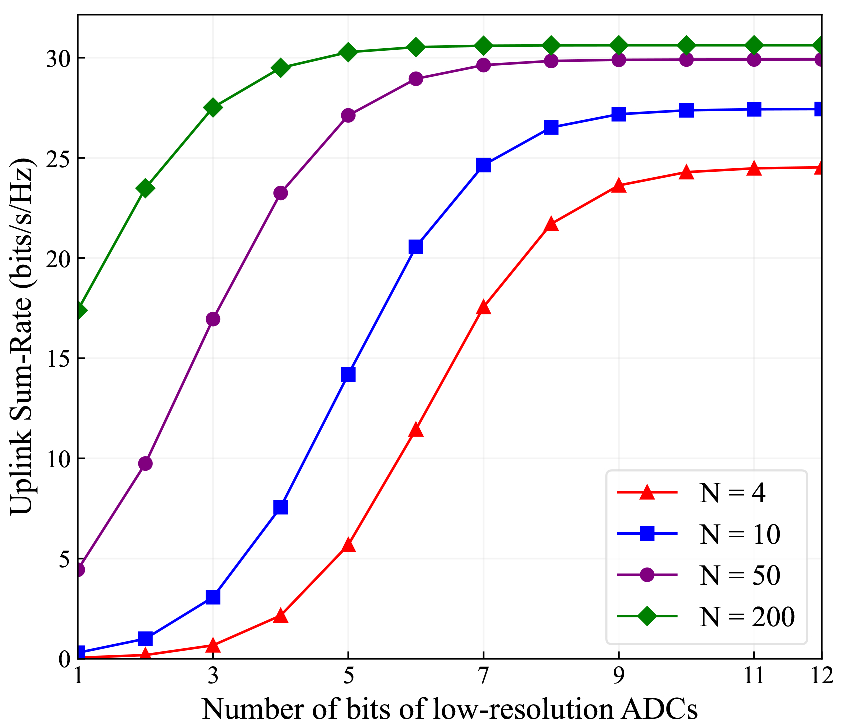
\includegraphics[width=2.7in] {fig5}
\caption{The relationship between uplink sum-rate and the number of bits of low resolution ADCs under different numbers of AP antennas, with $M$ = 100, $K$ = 20.}
\label{fig5}
\end{figure}

Figs. \ref{fig5} and \ref{fig6} respectively show the impact of low-resolution ADCs bit resolution on the uplink user sum-rate in the presence of several influencing factors. In each experiment, we assume that all APs are equipped with ADCs of the same resolution. It is evident that increasing the ADC resolution can significantly improve the user rate in both graphs before reaching the maximum value. Nevertheless, on a larger scale, the number of APs emerges as the primary determinant of user rate, indicating that increasing the number of APs can offset the rate loss caused by low-resolution ADCs. Furthermore, insufficient antennas result in a failure to achieve the maximum potential for the user rate. As shown in Fig. \ref{fig5}, the user rate approaches its limit only when $N \ge  50$, emphasizing the necessity of adjusting the number of antennas in accordance with the number of deployed APs in practical deployments to fully realize the potential of the system. Concurrently, as the quantity of antennas increases, the per-user rate gradually attains the upper limit of $1.5$ bits/s/Hz, which coincides with the presented insights. As $N$ becomes progressively larger in relation to ${\rho _\text{u}}\mathop \sum \limits_{m = 1}^M {\alpha _m}(1 - {\alpha _m})\left( {\mathop \sum \limits_{k = 1}^K {\beta _{mk}}\Omega _k + 1} \right){\gamma _{mk}}$, its effect on the user rate diminishes. Furthermore, the near-identical peak rates observed in Figs. \ref{fig5} and \ref{fig6} indicate that enhancing the resolution of ADCs and the number of AP antennas cannot exceed the intrinsic rate constraints of the system.

Subsequently, we undertake a comparative analysis of the achievable user rates in a CF-mMIMO system under both ideal and non-ideal hardware conditions, with varying numbers of APs and AP antennas. As illustrated in Fig. \ref{fig7}, under ideal conditions, the user sum-rate can reach a maximum of over 90 bits/s/Hz with an increase in the number of APs and AP antennas. However, the peak user sum-rate is constrained to approximately 30 bits/s/Hz due to the influence of nonlinear PAs and low-resolution ADCs. The presence of hardware impairments has been shown to result in a nearly $70\%$ reduction in user rates, which underscores the necessity for further investigation into systems with such impairments.
\begin{figure}
\centering

\includegraphics[width=3.2in] {fig6}
\caption{The impact of ADC bit count and AP count on uplink sum-rate, with $K$ = 20.}
\label{fig6}
\end{figure}
\begin{figure}
\centering

\includegraphics[width=3.2in] {fig7}
\caption{Comparing the uplink sum-rate in a CF-mMIMO system with nonlinear PAs and low-resolution ADCs versus the ideal hardware scenario, with $b_m$ = 10.}
\label{fig7}
\end{figure}
\begin{figure}
\centering
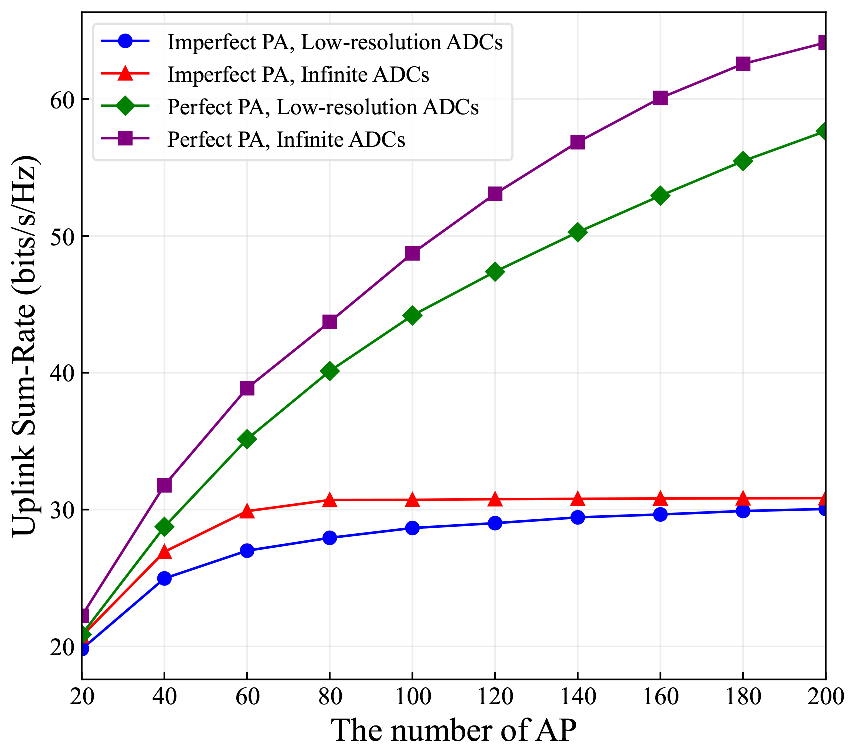
\includegraphics[width=2.7in] {compare}
\caption{Rate comparison based on different hardware impairments, with $b_m$ = 10, $K$ = 20.}
\label{compare}
\end{figure}

In order to delve deeper into the main factors that lead to significant user rate degradation, Fig. \ref{compare} designs a comparative experiment by manipulating hardware impairment variables. The experimental results show that under the ideal condition of assuming that the ADC has infinite resolution, the nonlinearity of the PA becomes a key constraint on the upper limit of the user rate, which strongly supports our insights into \eqref{eqn-23}. 

Next, we employ the proposed algorithms to finely calibrate the experimental parameters of each AP and UE in the entire system, demonstrating the performance improvements achieved by the algorithms from different perspectives. Fig. \ref{fig10} shows the optimization performance of the DMAGNN-AC algorithm compared to the full power transmission strategy and DDPG algorithm. The DDPG algorithm gradually approaches the optimal solution through interaction and exploration with the environment. After reaching the performance limit of the full power strategy, the per-user rate can be increased by an additional $2.8$ bit/s/Hz. In addition, after introducing DMAGNN as a feature extraction module, the cumulative distribution of rates is shifted to the right relative to DDPG. This confirms the ability of DMAGNN to enhance algorithm convergence and improve minimum user rate through interference modeling and multi-scale feature fusion. The comparison results under different AP-UE configurations show that the maximum user rate of the system is stable at about $3.8$ bit/s/Hz, representing the final performance boundary of user rate.

As shown in Fig. \ref{fig11}, under the assumption of maintaining a constant total number of bits, the proposed MADQIN algorithm provides a notable improvement in performance compared to the average allocation strategy. With an increase in the number of antennas, the user rates exhibit a gradually rising trend. It is noteworthy that adjusting the ADC resolution of the APs yields only smaller gains. This phenomenon can be attributed to the observation that, as illustrated in equation \eqref{eqn-23}, the rate is predominantly influenced by the total ADC resolution, irrespective of whether the signal in question is the desired signal or inter-user interference. Only the ADC quantization noise term demonstrates an impact associated with varying ADC resolutions. Therefore, this effect remains within an acceptable range.

Figs. \ref{fig8} and \ref{fig9} respectively show the loss values of the two algorithms during the iteration process. To make the results more universal, we compare the three loss results. It can be seen that both algorithms show a clear convergence trend after 1200 iterations. This observation strongly proves that both algorithms have excellent performance stability.
\begin{figure}
\centering

\includegraphics[width=2.7in] {fig10}
\caption{Comparison of per-user rate between full power transmission, DDPG$\_$Based, and DMAGNN-AC algorithm, with $b_m$ = 10, $N$ = 4.}
\label{fig10}
\end{figure}
\begin{figure}
\centering

\includegraphics[width=2.7in] {fig11}
\caption{Comparison of average allocation and the MADQIN algorithm under the same total bit count, with $b_\text{total}$ =135, $M$ = 15, and $K$ = 5.}
\label{fig11}
\end{figure}


\section{Conclusion}
In this paper, we studied uplink data transmission in a CF-mMIMO system in the presence of nonlinear PAs and low-resolution ADCs, and derived the closed-form expressions of achievable user rates. Our findings indicated that the performance of the system can be significantly affected by the quality of the hardware. To offset the decline in rate resulting from nonlinear PAs and low-resolution ADCs, we developed a DRL-based DMAGNN-AC power control algorithm to mitigate interference from other users. Compared with the full power transmission strategy and DDPG algorithm, this algorithm significantly improved system performance and the lower bound of minimum user rate. Subsequently, we utilized the MADQIN algorithm to appropriately adjust the ADC resolution, leading to a marginal improvement in user rate. Finally, the DRL algorithm validated the feasibility of employing low-quality hardware in CF-mMIMO systems.

\begin{figure}
\centering

\includegraphics[width=2.7in] {fig8}
\caption{Convergence of DMAGNN-AC algorithm.}
\label{fig8}
\end{figure}
\begin{figure}
\centering

\includegraphics[width=2.7in] {fig9}
\caption{Convergence of MADQIN algorithm.}
\label{fig9}
\end{figure}

\section*{Appendix \\Proof Of The Theorem 1}
For the formula \eqref{eqn-22}, we first calculate the expected signal $\text{ES}_k$. Since $\mathbf{\tilde{g} } _{mk}$ and $\mathbf{\hat{g}  } _{mk}$ are independent, we have
\begin{align}
{\text{ES}_k} &= { {\sqrt {{\rho _\text{u}}} \mathbb{E} \left\{ {\sum_{m = 1}^M {\alpha _m}({\tilde{a}_{1k}}{\bf{\hat g}}_{mk}^H{{\bf{g}}_{mk}} + {\tilde{a}_{3k}}{\bf{\hat g}}_{mk}^H{{\bf{g}}_{mk}}{{\left| {{q_k}} \right|}^2})} \right\}} }\nonumber\\
 &= \sqrt{\rho _\text{u}}\mathbb{E} \left \{ \sum_{m = 1}^M \alpha _m{\tilde{a}_{1k}}{\bf{\hat g}}_{mk}^H({{{\bf{\hat g}}}_{mk}} + {{\bf{\tilde g}}_{mk}}) \right \}\nonumber \\
 & \quad + \sqrt{\rho _\text{u}}\mathbb{E}\left \{  {\sum_{m=1}^{M}}\alpha _m{\tilde{a}_{3k}}{\bf{\hat g}}_{mk}^H({{{\bf{\hat g}}}_{mk}} + {\bf{\tilde g}}_{mk}{{\left| {{q_k}} \right|}^2})   \right \} \nonumber \\
 &= \sqrt {{\rho _\text{u}}} {{\mathbb{E} \left\{ {\sum_{m = 1}^M {\alpha _m}(N{\tilde{a}_{1k}}{\gamma _{mk}} + N{\tilde{a}_{3k}}{\gamma _{mk}}{{\left| {{q_k}} \right|}^2})} \right\}}}\nonumber\\
 &= {N}\sqrt{\rho _\text{u}}{\left| {{\tilde{a}_{1k}} + {\tilde{a}_{3k}}} \right|}{\sum_{m = 1}^M {\alpha _m}{\gamma _{mk}}}.
\end{align}

Besides, the variance of the additive noise $\text{N}_k$ is
\begin{align}\label{eqn-46}
\mathbb{E}\left\{\left|\text{N}_{k}\right|^{2}\right\}&=\sum_{m=1}^{M} \mathbb{E}\left\{\alpha_{m}^{2}\left\|\hat{\mathbf{g}}_{m k}\right\|^{2}\right\} \mathbb{E}\left\{\left\|\mathbf{w}_{\text{u}, m}\right\|^{2}\right\}\nonumber\\
&=N^{2} \sum_{m=1}^{M} \alpha_{m}^{2} \gamma_{m k}.
\end{align}

In addition, the variance of quantization noise is
\begin{equation}\begin{aligned}
\mathbb{E}\left\{ {{{\left| {{\text{Q}_k}} \right|}^2}} \right\} &= \mathbb{E}\left\{ {\left| {\mathop \sum \limits_{m = 1}^M {\bf{\hat g}}_{mk}^H{\bf{\tilde w}}_{\text{u},m}} \right|^2} \right\}\\
 %&= \mathop \sum \limits_{m = 1}^M \mathbb{E}\left\{ {{{\bf{\hat g}}_{mk}^H\bf{\tilde w}}_{\text{u},m}{\bf{\tilde w}}_{\text{u},m}^H\mathbf{\hat{g} }_{mk}}  \right\}\\
 &= N\sum_{m=1}^{M}\alpha_m (1-\alpha_m )\mathbb{E} \left \{ \mathbf{y}_{\text{u},m} \mathbf{y}_{\text{u},m}^H \right \} \gamma _{mk} \\
 &= {N}{\rho _\text{u}}\mathop \sum \limits_{m = 1}^M {\alpha _m}(1 - {\alpha _m})\left( {\mathop \sum \limits_{k = 1}^K {\beta _{mk}}\Omega _k + 1} \right){\gamma _{mk}}.
\end{aligned}\end{equation}

To facilitate the expansion of the formula, we define the total interference suffered by the $k$-th UE as $\Theta_k$, and the interference from other UEs as $\text{UI}_{kk'} \triangleq \text{I}_{kk'} + \text{NB}_{kk'}$. Therefore, the variance of the total interference can be expressed as 
\begin{align}\label{eqn-47}\mathbb{E } \left\{ {{{\left| \Theta_k  \right|}^2}} \right\} = \mathbb{E } \left\{ {{{\left| {\text{BU}_k} \right|}^2}{{\left| {{q_k}} \right|}^2} + \text{BU}_k^ * q_k^ * \sum _{l' \ne k}^K \text{UI}_{kl'}{q_{l'}}} \right\} \nonumber\\
+ \mathbb{E } \left\{ {\text{BU}_k{q_k}\sum_{k' \ne k}^K \text{UI}_{kk'}^ * q_{k'}^ *  + \sum_{k'l' \ne k}^K \text{UI}_{kk'}^ * \text{UI}_{kl'}q_{k'}^ * {q_{l'}}} \right\}.\end{align}

In the following, we calculate the values of the four terms in \eqref{eqn-47} separately.
The first term in \eqref{eqn-47} is decomposed into
\begin{align}\label{eqn-48}\mathbb{E}\left\{ {{{\left| {\text{BU}_k} \right|}^2}{{\left| {{q_k}} \right|}^2}} \right\} &\triangleq \mathbb{E}\left\{ {{{\text{B}_1}{\left| {{q_k}} \right|}^2}} \right\} - \mathbb{E}\left\{ {{{\text{B}_2}{\left| {{q_k}} \right|}^2}} \right\} \nonumber \\
&\quad- \mathbb{E}\left\{ {{{\text{B}_3}{\left| {{q_k}} \right|}^2}} \right\} + \mathbb{E}\left\{ {{{\text{B}_4}{\left| {{q_k}} \right|}^2}} \right\},\end{align}
where
\begin{align}{\text{B}_1} &= {\rho _\text{u}} { \mathop\sum\nolimits_{m = 1}^M {\alpha _m}\left(\tilde{a}_{1k}{{{\bf{\hat g}}}_{mk}}{\bf{g}}_{mk}^H + \tilde{a}_{3k}{{{\bf{\hat g}}}_{mk}}{\bf{g}}_{mk}^H{{\left| {{q_k}} \right|}^2}\right)}\nonumber \\
&\quad \times{\mathop\sum\nolimits_{n = 1}^M {\alpha _n}\left({\tilde{a}_{1k}}{\bf{\hat g}}_{nk}^H{{\bf{g}}_{nk}} + {\tilde{a}_{3k}}{\bf{\hat g}}_{nk}^H{{\bf{g}}_{nk}}\left | q_k \right |^2 \right)}\nonumber\\
&={N^2}{\rho _\text{u}} {\textstyle \sum_{m=1}^{M}}  {\Omega _{k'} \alpha _m^2{\gamma _{mk}}{\beta _{mk'}}},\end{align}
\begin{align}{\text{B}_2} &= {\rho _\text{u}} {\mathop \sum \nolimits_{m = 1}^M {\alpha _m}\left(\tilde{a}_{1k}{{{\bf{\hat g}}}_{mk}}{\bf{g}}_{mk}^H + \tilde{a}_{3k}{{{\bf{\hat g}}}_{mk}}{\bf{g}}_{mk}^H{{\left| {{q_k}} \right|}^2}\right)}\nonumber \\
&\quad \times {\mathop \sum \nolimits_{{\rm{m}} = 1}^M {\alpha _m}\left({\tilde{a}_{1k}}{\bf{\hat g}}_{mk}^H{{\bf{g}}_{mk}} + {\tilde{a}_{3k}}{\bf{\hat g}}_{mk}^H{{\bf{g}}_{mk}}\left | q_k \right |^2 \right)}\nonumber\\
&=N^2\rho _u {\textstyle \sum_{m=1}^{M}} \alpha _m^2\left ( \tilde{a}_{1k}^2\gamma _{mk}^2+3\tilde{a}_{1k}\tilde{a}_{3k}\gamma _{mk}^2 +2\tilde{a}_{3k}\gamma _{mk}^2   \right ) , \end{align}
\begin{equation}\begin{aligned}{\text{B}_3} = \text{B}_2^*,\end{aligned}\end{equation}
\begin{align}{\text{B}_4} &= {\rho _\text{u}}{\left| {\mathbb{E}\left\{ {\mathop \sum \nolimits_{m = 1}^M {\alpha _m}\left({\tilde{a}_{1k}}{\bf{\hat g}}_{mk}^H{{\bf{g}}_{mk}} + {\tilde{a}_{3k}}{\bf{\hat g}}_{mk}^H{{\bf{g}}_{mk}}{{\left| {{q_k}} \right|}^2}\right)} \right\}} \right|^2}\nonumber\\
&=N^2\rho _u\left | {\tilde{a}_{1k}} + {\tilde{a}_{3k}} \right |^2 { {\textstyle \sum_{m=1}^{M}}  {\alpha _m}^2{\gamma _{mk}^2}}.\end{align}

The raw data $q_k$ is a circularly symmetric complex Gaussian random variable and $\mathbb{E} \{ \left | q_k \right |^2 \} =1, \mathbb{E}  \{ \left | q_k \right |^4  \} =2,\mathbb{E} \{ \left | q_k \right |^6 \} =6$. When $k' \ne k$ in the second and third items of \eqref{eqn-47}, the intersection of ${q_{k'}}$ and ${q_k}$ leads to
\begin{equation}\begin{aligned}\mathbb{E}\left\{ {\text{BU}_k^ * q_k^ * \sum _{l' \ne k}^K\text{UI}_{kl'}{q_{l'}}} \right\} = \mathbb{E}\left\{ {\text{BU}_k{q_k}\sum _{k' \ne k}^K\text{UI}_{kk'}^ * q_{k'}^ * } \right\} = \mathbf{0} .\end{aligned}\end{equation}

In the fourth item of \eqref{eqn-47}, let $\text{UI}_{kk'}^H\text{UI}_{kl'} = {\text{U}_1} + {\text{U}_2} + {\text{U}_3} + {\text{U}_4}$. Subsequently, the results are presented as follows
\begin{equation}\begin{aligned}\label{eqn-54}\mathbb{E}\left\{ {\mathop \sum \limits_{k',l' \ne k}^K {\text{U}_1}q_{k'}^ * {q_{l'}}} \right\} = {N^2}{\rho _\text{u}}\mathop \sum \limits_{k' \ne k}^K \mathop \sum \limits_{m = 1}^M \alpha _m^2{\left| {{\tilde{a}_{1k'}}} \right|^2}{\gamma _{mk}}{\beta _{mk'}},\end{aligned}\end{equation}
\begin{equation}\begin{aligned}\mathbb{E}\left\{ {\mathop \sum \limits_{k',l' \ne k}^K {\text{U}_2}q_{k'}^ * {q_{l'}}} \right\} = 2{N^2}{\rho _\text{u}}\mathop \sum \limits_{k' \ne k}^K \mathop \sum \limits_{m = 1}^M \alpha _m^2\tilde{a}_{1k'}^ * {\tilde{a}_{3k'}}{\gamma _{mk}}{\beta _{mk'}},\end{aligned}\end{equation}
\begin{equation}\begin{aligned}\mathbb{E}\left\{ {\mathop \sum \limits_{k',l' \ne k}^K {\text{U}_3}q_{k'}^ * {q_{l'}}} \right\} = 2{N^2}{\rho _\text{u}}\mathop \sum \limits_{m = 1}^M \mathop \sum \limits_{k' \ne k}^K \alpha _m^2{\tilde{a}_{1k'}}\tilde{a}_{3k'}^ * {\gamma _{mk}}{\beta _{mk'}},\end{aligned}\end{equation}
\begin{equation}\begin{aligned}\label{eqn-57}\mathbb{E}\left\{ {\mathop \sum \limits_{k',l' \ne k}^K {\text{U}_4}q_{k'}^ * {q_{l'}}} \right\} = 6{N^2}{\rho _\text{u}}\mathop \sum \limits_{m = 1}^M \mathop \sum \limits_{k' \ne k}^K {\left| {{\tilde{a}_{3k'}}} \right|^2}\alpha _m^2{\gamma _{mk}}{\beta _{mk'}}.\end{aligned}\end{equation}

Combining \eqref{eqn-54}-\eqref{eqn-57}, we can obtain
\begin{equation}\begin{aligned}\mathbb{E}\left\{ {\mathop \sum \limits_{k',l' \ne k}^k \text{UI}_{kk'}^ * \text{UI}_{kl'}q_{k'}^ * {q_{l'}}} \right\} = {N^2}{\rho _\text{u}}\mathop \sum \limits_{m = 1}^M {\mathop \sum \limits_{k' \ne k}^K\Omega _{k'} \alpha _m^2{\gamma _{mk}}{\beta _{mk'}}}. \end{aligned}\end{equation}


To this end, the proof of \textit{Theorem 1} has been completed.



\begin{thebibliography}{99}
\bibitem{paperI1}
K. Samdanis and T. Taleb, “The road beyond 5G: A vision and insight of the key technologies,” \textit{IEEE Netw.}, vol. 34, no. 2, pp. 135-141, Feb. 2020.

\bibitem{paperI2}
V. Ziegler, H. Viswanathan, H. Flinck, M. Hoffmann, V. Räisänen, and K. Hätönen, “6G architecture to connect the worlds,” \textit{IEEE Access}, vol. 8, pp. 173508-173520, Sept. 2020.

\bibitem{paperI3}
H. Q. Ngo, A. Ashikhmin, H. Yang, E. G. Larsson, and T. L. Marzetta, “Cell-free massive MIMO versus small cells,” \textit{IEEE Trans. Wireless Commun.}, vol. 16, no. 3, pp. 1834–1850, Mar. 2017.

\bibitem{paperI4}
O. T. Demir, E. Björnson, and L. Sanguinetti, “Foundations of usercentric cell-free massive MIMO,” \textit{Found. Trends Signal Process.}, vol. 14, no. 3–4, pp. 162–472, 2021.

\bibitem{paperI5}
G. Interdonato, E. Björnson, H. Q. Ngo, P. Frenger, and E. G. Larsson, “Ubiquitous cell-free massive MIMO communications,” \textit{EURASIP J. Wireless Commun. Netw.}, vol. 2019, no. 1, pp. 1–13, Dec. 2019.

\bibitem{paperI6}
S. -N. Jin, D. -W. Yue, and H. H. Nguyen, “Spectral and energy efficiency in cell-free massive MIMO systems over correlated Rician fading,” \textit{IEEE Syst. J.}, vol. 15, no. 2, pp. 2822–2833, Jun. 2021.

\bibitem{paperI7}
H. Q. Ngo, L. -N. Tran, T. Q. Duong, M. Matthaiou, and E. G. Larsson, “On the total energy efficiency of cell-free massive MIMO,” \textit{IEEE Trans. Green Commun. Netw.}, vol. 2, no. 1, pp. 25–39, Mar. 2018.

\bibitem{paperI8}
E. Nayebi, A. Ashikhmin, T. L. Marzetta, H. Yang, and B. D. Rao, “Precoding and power optimization in cell-free massive MIMO systems,” \textit{IEEE Trans. Wireless Commun.}, vol. 16, no. 7, pp. 4445–4459, Jul. 2017.

\bibitem{paperI9}
L. D. Nguyen, T. Q. Duong, H. Q. Ngo, and K. Tourki, “Energy effi-ciency in cell-free massive MIMO with zero-forcing precoding design,” \textit{IEEE Commun. Lett.}, vol. 21, no. 8, pp. 1871–1874, Aug. 2017.

\bibitem{paperIA15}
Y. Zhang, M. Zhou, Y. Cheng, L. Yang, and H. Zhu, “RF impairments and low-resolution ADCs for nonideal uplink cell-free massive MIMO systems,” \textit{IEEE Syst. J.}, vol. 15, no. 2, pp. 2519-2530, Jun. 2021.

\bibitem{paperI10}
S. Chen, J. Zhang, J. Zhang, E. Björnson, and B. Ai, “A survey on user-centric cell-free massive MIMO systems,” 2021, \textit{arXiv:2104.13667}. [Online]. Available: http://arxiv.org/abs/2104.13667.

\bibitem{paperI11}
J. Choi and B. L. Evans, “Analysis of ergodic rate for transmit antenna selection in low-resolution ADC systems,” \textit{IEEE Trans. Veh. Technol.}, vol. 68, no. 1, pp. 952-956, Jan. 2019.

\bibitem{paperI12}
H. He, C. -K. Wen, and S. Jin, “Bayesian optimal data detector for hybrid mmWave MIMO-OFDM systems with low-resolution ADCs,” \textit{IEEE J. Sel. Topics Signal Process.}, vol. 12, no. 3, pp. 469-483, Jun. 2018.

\bibitem{paperI13}
S. -N. Hong, S. Kim, and N. Lee, “A weighted minimum distance decoding for uplink multiuser MIMO systems with low-resolution ADCs,” \textit{IEEE Trans. Commun.}, vol. 66, no. 5, pp. 1912-1924, May 2018.

%IA
\bibitem{paperIA1}
J. Zhang, Y. Wei, E. Björnson, Y. Han, and S. Jin, “Performance analysis and power control of cell-free massive MIMO systems with hardware impairments,” \textit{IEEE Access}, vol. 6, pp. 55302-55314, Sept. 2018.

\bibitem{paperIA2}
M. Xie, X. Yu, Y. Rui, K. Wang, X. Dang, and J. Zhang, “Performance analysis for user-centric cell-free massive MIMO systems with hardware impairments, and multi-antenna users,” \textit{IEEE Trans. Wireless Commun.}, vol. 23, no. 2, pp. 1243-1259, Feb. 2024.

\bibitem{paperIA3}
B. Lim, W. J. Yun, J. Kim, and Y. -C. Ko, “Joint pilot design and channel estimation using deep residual learning for multi-cell massive MIMO under hardware impairments,” \textit{IEEE Trans. Veh. Technol.}, vol. 71, no. 7, pp. 7599-7612, Jul. 2022.

\bibitem{paperIA4}
Y. Zhang, Q. Zhang, H. Hu, L. Yang, and H. Zhu, “Cell-free massive MIMO systems with non-ideal hardware: Phase drifts and distortion noise,” \textit{IEEE Trans. Veh. Technol.}, vol. 70, no. 11, pp. 11604-11618, Nov. 2021.


\bibitem{paperIA5}
S. Jacobsson, U. Gustavsson, G. Durisi, and C. Studer, “Massive MU-MIMO-OFDM uplink with hardware impairments: Modeling and analysis,” in \textit{Proc. Asilomar Conf. Signals, Syst. Comput. (ACSSC)}, Pacific Grove, CA, USA, 2018, pp. 1829-1835.

\bibitem{paperIA6}
E. Björnson, J. Hoydis, M. Kountouris, and M. Debbah, “Massive MIMO systems with non-ideal hardware: Energy efficiency, estimation, and capacity limits,” \textit{IEEE Trans. Inf. Theory.}, vol. 60, no. 11, pp. 7112-7139, Nov. 2014.

\bibitem{paperIA7}
E. Björnson, J. Hoydis, and L. Sanguinetti, “Massive MIMO networks: Spectral, energy, and hardware efficiency,” \textit{Found. Trends Signal Process.}, 2017.

\bibitem{paperIA8}
Q. Sun, X. Ji, Z. Wang, X. Chen, Y. Yang, J. Zhang, and K. Wong, “Uplink performance of hardware-impaired cell-free massive MIMO with multi-antenna users and superimposed pilots,” \textit{IEEE Trans. Commun.}, vol. 71, no. 11, pp. 6711-6726, Nov. 2023.

\bibitem{paperIA9}
X. Hu, C. Zhong, X. Chen, W. Xu, H. Lin, and Z. Zhang, “Cell-free massive MIMO systems with low resolution ADCs,” \textit{IEEE Trans. Commun.}, vol. 67, no. 10, pp. 6844-6857, Oct. 2019.

\bibitem{paperIA10}
Y. Zhang, M. Zhou, X. Qiao, H. Cao, and L. Yang, “On the performance of cell-free massive MIMO with low-resolution ADCs,” \textit{IEEE Access}, vol. 7, pp. 117968-117977, Aug. 2019.

\bibitem{paperIA11}
M. Zhou, L. Yang, and H. Zhu, “Sum-SE for multigroup multicast cell-free massive MIMO with multi-antenna users and low-resolution DACs,” \textit{IEEE Wireless Commun. Lett.}, vol. 10, no. 8, pp. 1702-1706, Aug. 2021.

\bibitem{paperIA12}
M. Zhou, J. Li, M. Xie, C. Zhang, and J. Yuan, “Average sum rate of D2D underlaid multigroup multicast cell-free massive MIMO with multi-antenna users,” \textit{IEEE Wireless Commun. Lett.}, vol. 12, no. 1, pp. 60-64, Jan. 2023.

\bibitem{paperIA16}
R. S. Sutton and A. G. Barto, \textit{Reinforcement learning: An introduction.} Cambridge, MA, USA: MIT Press, 2018.

\bibitem{paperIA17}
F. Meng, P. Chen, L. Wu, and J. Cheng, “Power allocation in multi-user cellular networks: Deep reinforcement learning approaches,” \textit{IEEE Trans. Wireless Commun.}, vol. 19, no. 10, pp. 6255-6267, Oct. 2020.

\bibitem{paper10} 
Y. Zhao, F. Zhang, Z. Zhou, and G. Hu, “A dynamic power allocation approach for downlink cell-free massive MIMO with graph neural network,” \emph{IEEE Trans. Veh. Technol.}, doi: 10.1109/TVT.2024.

\bibitem{paperIB3}
Z. Liu, J. Zhang, E. Shi, Z. Liu, D. Niyato, B. Ai, and X. S. Shen, “Graph neural network meets multi-agent reinforcement learning: Fundamentals, applications, and future directions,” \emph{IEEE Wireless Commun.}, vol. 31, no. 6, pp. 39-47, Dec. 2024.

\bibitem{paperIB4}
Y. Shen, J. Zhang, S. H. Song, and K. B. Letaief, “Graph neural networks for wireless communications: From theory to practice,” \emph{IEEE Trans.
Wireless Commun.}, vol. 22, no. 5, pp. 3554–3569, May 2023.

%正文文献
\bibitem{paper1}
U. Gustavsson, C. Sanchéz-Perez, T. Eriksson, F. Athley, G. Durisi, and P. Landin, “On the impact of hardware impairments on massive MIMO,” in \emph{Proc. IEEE Globecom Workshops (GC Wkshps)}, Austin, TX, USA, 2014, pp. 294–300.

\bibitem{paper2}
A. Mohammadi and F. M. Ghannouchi, \textit{RF transceiver design for MIMO wireless communications.} Springer Science \& Business Media, 2012, vol. 145.

\bibitem{paper3}
D. Rönnow and P. Händel, “Nonlinear distortion noise and linear attenuation in MIMO systems—Theory and application to multiband transmitters,” \emph{IEEE Trans. Signal Process.}, vol. 67, no. 20, pp. 5203–5212, Oct. 2019.

\bibitem{paper4}
P. Händel and D. Rönnow, “Dirty MIMO transmitters: Does it matter?” \emph{IEEE Trans. Wireless Commun.}, vol. 17, no. 8, pp. 5425–5436, Aug. 2018.

\bibitem{paper5}
Ö. T. Demir and E. Björnson, “Channel estimation in massive MIMO under hardware non-linearities: Bayesian methods versus deep learning,” \emph{IEEE Open J. Commun. Soc.}, vol. 1, pp. 109-124, Dec. 2020.

\bibitem{paper6}
M. Jadidi, A. M. Khoueini, A. Mohammadi, and V. Meghdadi, “Performance analysis and power allocation for uplink cell-free massive MIMO system with nonlinear power amplifier,” \emph{IEEE Trans. Commun.}, vol. 72, no. 9, pp. 5473-5485, Sept. 2024.

\bibitem{paper7}
J. Zhang, L. Dai, S. Sun, and Z. Wang, “On the spectral efficiency of massive MIMO systems with low-resolution ADCs,” \textit{IEEE Commun. Lett.}, vol. 20, no. 5, pp. 842-845, May 2016.

\bibitem{paper8}
J. Zhang, L. Dai, Z. He, S. Jin, and X. Li, “Performance analysis of mixed-ADC massive MIMO systems over rician fading channels,” \textit{IEEE J. Sel. Areas Commun.}, vol. 35, no. 6, pp. 1327-1338, Jun. 2017.

\bibitem{paper9}
J. Yuan, S. Jin, C. -K. Wen, and K. -K. Wong, “The distributed MIMO scenario: Can ideal ADCs be replaced by low-resolution ADCs?,” \textit{IEEE Wireless Commun. Lett.}, vol. 6, no. 4, pp. 470-473, Aug. 2017.

\bibitem{paper11}
S. Mishra, L. Salaun, H. Yang, and C. S. Chen, “Graph neural network aided power control in partially connected cell-free massive MIMO,” \emph{IEEE Trans. Wireless Commun.}, vol. 23, no. 9, pp. 12412-12423, Sept. 2024.

\bibitem{paper12}
Z. Liu, J. Zhang, Y. Zhu, E. Shi, and B. Ai, “Mobile cell-free massive MIMO with multi-agent reinforcement learning: A scalable framework,” \emph{IEEE Trans. Wireless Commun.}, doi: 10.1109/TWC.2024.

\bibitem{paper13} 
P. Velickovic, G. Cucurull, A. Casanova, A. Romero, P. Lio, and Y. Bengio, “Graph attention networks”, 2018, \emph{arXiv:1710.10903.} [Online]. Available: https://arxiv.org/abs/1710.10903.

\bibitem{paper14} 
M. Eisen and A. Ribeiro, “Optimal wireless resource allocation with random edge graph neural networks,” \emph{IEEE Trans. Signal Process.}, vol. 68, pp. 2977-2991, Apr. 2020.

\bibitem{paper15}
H. Moazzen, A. Mohammadi, and M. Majidi, “Performance analysis of linear precoded MU-MIMO-OFDM systems with nonlinear power amplifiers and correlated channel,” \textit{IEEE Trans. Commun.}, vol. 67, no. 10, pp. 6753-6765, Oct. 2019.










\end{thebibliography}

\end{CJK}
\end{document}


